%%%%%%%%%%%%%%%%%%%-D O  N O T  D E L E T E-%%%%%%%%%%%%%%%%%%%%
%%%%%%%%%%%%%%%%%%%%%%%%%%%%%%%%%%%%%%%%%%%%%%%%%%%%%%%%%%%%%%%%
%%                                                            %%
%%  BulSU BS Math Thesis Proposal                             %%
%%  LateX Template                                            %%
%%  Version 4 (4 November 2024)                               %%
%%                                                            %%
%%  Load documentclass{bulsuthesis}                           %%
%%  This template is for the use of BS Math students of       %%
%%  the Collge of Sicence, Bulacan State University           %%
%%  in typsetting their undergraduate thesis.                 %%
%%                                                            %%
%%  Original Author:                                          %%
%%  Harris R. Dela Cruz                                       %%
%%  Bulacan State University                                  %%
%%  e-mail: harris.delacruz@bulsu.edu.ph                      %%
%%                                                            %%
%%  Permission: Any student of the University is hereby given %%
%%  permission to use this template and the accompanying      %%
%%  bulsuthesis.cls and thesis-structure.tex files provided   %%
%%  the original author is given due acknwledgement.          %%
%%                                                            %%
%%%%%%%%%%%%%%%%%%%%%%%%%%%%%%%%%%%%%%%%%%%%%%%%%%%%%%%%%%%%%%%%
%%%%%%%%%%%%%%%%%%%-D O  N O T  D E L E T E-%%%%%%%%%%%%%%%%%%%%

\documentclass[hidelinks,a4paper,12pt]{bulsuthesis}
\usepackage{lipsum}			%garbage words
\usepackage[none]{hyphenat} 	%no hypenation
%----------------------------------------------------------------
% SECTIONING FORMAT
%----------------------------------------------------------------
%\usepackage[skip=5ex]{parskip}
\setcounter{secnumdepth}{0}	%<-section numbering only up to sec
	%\titleformat{command}[shape]{format}{label}{sep}{before-code}[after-code]

\titleformat{\chapter}[display]
	{\centering\normalfont\normalsize\bfseries}
	{\MakeUppercase{\chaptertitlename\ \thechapter}\filcenter}
	{0pt}%sep
	{\centering\uppercase}
	{\normalsize\filcenter}
\titlespacing{\chapter}{0pt}{-27pt}{18pt}
\renewcommand{\thechapter}{\Roman{chapter}}

\titleformat{\section}
	{\normalfont\normalsize\bfseries}
	{\thesection}
	{1em}
	{}
\renewcommand{\thesection}{\arabic{chapter}.\arabic{section}}
\titlespacing{\section}{0pt}{2ex plus 1ex minus 0ex}{0ex}

\titleformat{\subsection}
	{\normalfont\normalsize\itshape\bfseries}
	{\thesubsection}
	{1em}
	{}
\titlespacing{\subsection}{0pt}{2ex plus 1ex minus 0ex}{0ex}

\titleformat{\subsubsection}
{\normalfont\normalsize\itshape}
{\thesubsubsection}
{1em}
{}
\titlespacing{\subsubsection}{0pt}{\parskip}{-\parskip}

\newenvironment{centerappendixtitle}%
{\begingroup
	\titlespacing{\chapter}{0pt}{.5\textheight-30pt}{18pt}
	\pagestyle{plain}
}{%
	\clearpage
	\titlespacing{\chapter}{0pt}{-27pt}{18pt}
	\pagestyle{fancy}
	\endgroup
}



%----------------------------------------------------------------
% TABLE/FIGURES/EQUATION
%----------------------------------------------------------------
\usepackage{booktabs,longtable,threeparttable,siunitx,tabularx,rotating,pdflscape,float}
\usepackage{array,multicol,multirow,color,calc,subcaption}
	\newcolumntype{L}[1]{>{\raggedright\let\newline\\\arraybackslash\hspace{0pt}}p{#1}}
	\newcolumntype{C}[1]{>{\centering\let\newline\\\arraybackslash\hspace{0pt}}p{#1}}
	\newcolumntype{R}[1]{>{\raggedleft\let\newline\\\arraybackslash\hspace{0pt}}p{#1}}
\usepackage{caption}
	\DeclareCaptionLabelSeparator*{spaced}{\\[1ex]}
	\renewcommand{\thetable}{\arabic{table}}
	\captionsetup[table]{
%		font=sf,
		labelfont=bf,
		textfont=it, 
		format=plain,
		justification=justified,
		singlelinecheck=false,
		labelsep=spaced,skip=12pt
		}
	\renewcommand{\thefigure}{\arabic{chapter}.\arabic{figure}}
	\captionsetup[figure]{
%		font=sf,
		labelfont=bf,
		textfont=it, 
		format=plain,
		justification=justified,
		singlelinecheck=false,
		labelsep=spaced,skip=12pt
		}
	\renewcommand{\theequation}{\arabic{chapter}.\arabic{equation}}
	
	\counterwithout{table}{chapter}
	\counterwithout{figure}{chapter}


%----------------------------------------------------------------
% TABLE OF CONTENTS
%----------------------------------------------------------------
%\usepackage[titles]{tocloft}
\setcounter{tocdepth}{1} 	%<-toc level shows only up to sec
%setting the indentation of section in the TOC
\setlength{\cftchapnumwidth}{2em}
\setlength{\cftsecindent}{2em}

\makeatletter
\renewcommand*\l@figure{\@dottedtocline{1}{1em}{3.5em}}% Default: 1.5em/2.3em
\let\l@table\l@figure
\makeatother

\makeatletter
\def\@chapter[#1]#2{\ifnum \c@secnumdepth >\m@ne
	\refstepcounter{chapter}%
	\typeout{\@chapapp\space\thechapter.}%
	\addcontentsline{toc}{chapter}%
	{\protect\numberline{\thechapter}\texorpdfstring{\uppercase{#1}}{#1}}%
	\else
	\addcontentsline{toc}{chapter}{\texorpdfstring{\uppercase{#1}}{#1}}%
	\fi
	\chaptermark{#1}%
	\addtocontents{lof}{\protect\addvspace{10\p@}}%
	\addtocontents{lot}{\protect\addvspace{10\p@}}%
	\if@twocolumn
	\@topnewpage[\@makechapterhead{#2}]%
	\else
	\@makechapterhead{#2}%
	\@afterheading
	\fi}
\makeatother

%----------------------------------------------------------------
% BIBLIOGRAPHY
%----------------------------------------------------------------
\usepackage[american]{babel}
\usepackage{csquotes}
\usepackage[style=apa,defernumbers=true]{biblatex}
	\DeclareLanguageMapping{american}{american-apa}
	\defbibheading{subbibliography}[\refname]{\section*{#1}}
\usepackage{hyperref}

\graphicspath{{Figures/}}	%change graphic path folder
\addbibresource{reference.bib} %filename of your .bib database
%\geometry{showframe}

%--------------------------------------------------------------%
% THESIS BASIC INFORMATION
%--------------------------------------------------------------%
\title{ Design and Implementation of a Shelter Location-Allocation System in Calumpit, Bulacan using Genetic Algorithm }%Type your thesis title here without any line break

\fronttitle{%
	Design and Implementation of a Shelter Location- 
	\protect\\Allocation System in Calumpit, Bulacan
	\protect\\Using Genetic Algorithm
	} 
	%Type your thesis title as how it will appear [inverted triangle] in the title page
	%Use \protect\\ to force a new line in the title

\author{%Name of the research proponents, in alphabetical order
	Bryan Jett T. Calulo
	
	Lovely Angeline OL. Cunanan
	
	Elijah Iñigo C. Fabian
	
}
\authorone{Bryan Jett T. Calulo}  %<-Re-type individual names here
\authortwo{Lovely Angeline OL. Cunanan}  %<-Re-type individual names here
\authorthree{Elijah Iñigo C. Fabian}%<-Re-type individual names here

\papertype{Thesis Proposal} %papertype can be thesis proposal, 
%thesis or dissertation
\adviser{Dr. Valentine Blez L. Lampayan, PhD.}		%<-thesis adviser
\panelchair{Panel Chair}	%<-thesis panel-chair
\paneltwo{Panel Member 2}		%<-thesis panel-member
\panelthree{Panel Member 3}		%<-thesis panel-member
\degree{Bachelor of Science in Mathematics} %<-student's course
\specialization{Computer Science} %<-student's specialization
\college{College of Science}	%<-student's college
\csdean{THELMA V. PAGTALUNAN, PhD.}%<-dean of the college
\ddate{December 2024}			%<-Month Year of defense date


\begin{document}
\emergencystretch 3em
\renewcommand{\contentsname}{TABLE OF CONTENTS}
\renewcommand{\listtablename}{LIST OF TABLES}
\renewcommand{\listfigurename}{LIST OF FIGURES}

%--------------------------------------------------------------%
% FRONTMATTER
%--------------------------------------------------------------%
\doublespacing
\begin{preliminary}
	\maketitle
	\tableofcontents 		%<-print the ToC
	\newpage
	\listoftables			%<-print the list of tables page
		\addcontentsline{toc}{chapter}{LIST OF TABLES}
		\addtocontents{lot}{\noindent\makebox[0.75in][l]{\textbf{Table}}\makebox[\linewidth-0.75in]{\textbf{Title}\hfill\textbf{Page}}\par}
	\newpage
	\listoffigures			%<-print the list of figures page
		\addcontentsline{toc}{chapter}{LIST OF FIGURES}
		\addtocontents{lof}{\noindent\makebox[0.75in][l]{\textbf{Figure}}\makebox[\linewidth-0.75in]{\textbf{Title}\hfill\textbf{Page}}\par}
	\newpage
\end{preliminary}

	\addtocontents{toc}{\let\protect\contentsline\protect\nopagecontentsline}
	\addcontentsline{toc}{chapter}{CHAPTER}
	\addtocontents{toc}{\let\protect\contentsline\protect\oldcontentsline}


%--------------------------------------------------------------%
% MAINMATTER
%--------------------------------------------------------------%
%Compose the body of your thesis in separate .tex file
%Input them separately using the command \input{filename}
\chapter{The Problem and Its Background}

	Addressing the shelter issues in Bulacan is the focus of this research. This chapter highlights the background and significance of the study. Additionally, the key points and objectives of the study are discussed along with the study's scope and limitations.

\section{Background of the Study}

	The Philippines experiences typhoons, earthquakes, and volcanic eruptions each year, leaving people vulnerable and displaced because the country is situated within the Pacific Ring of Fire and directly in the path of the typhoon belt in the Pacific Ocean. Bulacan itself has faced severe impacts from typhoons, including Typhoon Ondoy in 2009 which affected over 250, 000 families and claimed nearly 100 lives  \parencite{James2009}. For instance, typhoon Haiyan, also known as Super Typhoon Yolanda, devastated the nation in 2013 and displaced over 4 million people, exposing severe shortcomings in the Philippine shelter allocation systems \parencite{Iuchi2019}, highlighting the urgent need for efficient and responsive disaster management strategies. Despite ongoing efforts, the country continues to face significant challenges in shelter allocation, like overcrowding, resource distribution inefficiencies, and poor accessibility.
	
	Overcrowding remains a persistent issue, with many shelters operating beyond their intended capacity, leading to unsafe and unsanitary conditions. Accessibility problems further worsen the situation, as shelters are often located at distances difficult for affected individuals, particularly those in rural or remote areas, to reach due to poor infrastructure.	Additionally, the inefficient distribution of resources like food, water, and medical supplies results in shortages and uneven support across shelters. Compounding these issues such as disaster preparedness team do not use data-driven decision-making increasing the likelihood of making incorrect decisions highlights the data and planning gaps that hinder effective decision-making and timely shelter assignments. This emphasizes the need on developing innovative approaches to improve shelter allocation in disaster preparedness. 
	
	The concept of shelter allocation has been a critical aspect of disaster management throughout history, when communities would seek refuge in caves or fortified structures during emergencies. However, formalized shelter allocation strategies emerged in the 20th century with the rise of civil defense measures during World War II, where air raid shelters were established in urban areas. These air raid shelters were used to ensure the safety of the population of Europe because of the civil casualties and weakening of their social and military morale, as seen in London, Berlin, and Paris \parencite{Flebus1941,Shakibamaesh2015}. Post-war, shelter allocation evolved in response to natural disasters, and humanitarian organizations developed temporary shelters for displaced populations. Later, in 1970 in Bangladesh, the inadequacy of early efforts became evident during the Bhola cyclone, which led to numerous deaths. A study showed that people lacked access to information about the cyclone warning and that appropriate shelters were rare, resulting in a devastating 300,000 fatalities, with some estimates being even higher and an estimated 4.8 million people were affected by the cyclone due to the lack of effective shelter allocation. \parencite{Mari2020}
	
	Shelter allocation refers to the process of assigning displaced communities to available shelters during disasters \parencite{Yin2023}. While shelter location-allocation,  focuses on determining shelter would be constructed, and then be used for displaced population \parencite{Xiujuan2019}. These process is crucial to disaster prevention and mitigation, ensuring the safety and well-being of affected populations by providing secure, accessible, and adequate temporary shelters. Effective shelter allocation involves considerations such as shelter capacity, proximity to disaster sites, and the specific needs of vulnerable communities. 
	
	Over the years, strategies have evolved from reactive measures to a more systematic approach incorporating modern technologies and methodologies, highlighting the increasing importance of structured and efficient shelter allocation. However, these challenges, particularly in developing countries like the Philippines, where limited infrastructure hinders its effective implementation.
	
	This study proposes a data-driven solution ensuring an effective and feasible implementation of shelter allocation. This would be by developing a decision support system using a genetic algorithm (GA), a computational method inspired by natural selection and evolution, to address the inefficiencies in shelter allocation. GA optimize solutions by mimicking the process of evolution such as selection, crossover, and mutation, to identify best outcome. \textcite{Mathew2012} discussed that these algorithms represent potential solutions to a given problem using a basic chromosome-like data structure and employ recombination operators to maintain essential information, making it ideal to solve wide variety of problems. In shelter allocation, GA can optimize the assignment process by simultaneously considering factors such as shelter capacity, location, and accessibility. This approach aims to minimize overcrowding, improve resource distribution, and enhance overall efficiency in managing shelters during disasters.
		
	Given the Philippines' frequent exposure to natural disasters, implementing a shelter allocation system is essential. Calumpit, Bulacan was chosen for its high vulnerability to flooding since it has been a catch basin of floodwaters from their neighboring areas. Despite the multitude of studies formulating models to address the shelter location-allocation problem, there remains a lack of system integration. This gap makes it difficult for decision-makers, particularly those unfamiliar with the mathematical models proposed in various studies, to apply them effectively in their decisions. This study is dedicated to developing a programmed system that uses genetic algorithm to address the challenges experienced in the Philippines, focusing on Calumpit, Bulacan. The proposed shelter location-allocation system has the potential to significantly improve disaster response efficiency, and enhance safety for displaced individuals.The insights gained from this study could be applied to other municipalities facing similar challenges, contributing to the national effort to strengthen disaster resilience. 
	%\nocite{*}.

\section{Statement of the Problem}
	This study aims to address the shelter allocation problem for the municipality of Calumpit, particularly during disaster situations such as storm surges and flash floods. The primary challenge is how to develop a decision support system integrating a model that solves location-allocation problem to ensure that victims are allocated to shelters in an optimal manner. Specifically, the paper aims to solve the following questions:
	
	\begin{enumerate}
		\item How can the proposed system be developed featuring the following functionalities:
		\begin{enumerate}[label*=\arabic*]
			\item Data Modification,
			\item Model Modification,
			\item Data Simulation,
			\item Shelter Tagging, and
			\item Report Protection?
		\end{enumerate}
		\item What is the optimal shelter location-allocation plan for the municipality of Calumpit?
		\item How acceptable is the proposed system based on the criteria defined in Technology Acceptance Model?
		\begin{enumerate}[label*=\arabic*]
			\item Perceived usefulness,
			\item Perceived ease of use,
			\item Attitude towards using, and
			\item Behavioral intention?
		\end{enumerate}
		\item How well does the proposed system meet the ISO / IEC 25010 requirements?
		\begin{enumerate}[label*=\arabic*]
			\item Functional Suitability,
			\item Performance Efficiency,
			\item Compatibility,
			\item Interaction Capability,
			\item Reliability,
			\item Security,
			\item Maintainability, and
			\item Flexibility?
		\end{enumerate}
	\end{enumerate}
	
\section{Significance of the Study}
	The research seeks to improve disaster preparedness by providing a program and a model that facilitates more efficient decision-making and optimizes shelter placements regarding accessibility, cost-efficiency, and community proximity.The proposed solution has the potential to significantly reduce the risks associated with natural disasters in that area and enhance the overall management of shelter allocation and emergency resources.
	
	The resulting shelter location-allocation from this project will primarily benefit the citizens of disaster-prone areas in Calumpit. This leads to faster evacuation times for use in the welfare of its citizens. The resulting optimization of shelter locations also extends to the efficient use of financial and logistical resources, minimizing the costs required in the maintenance and operation of shelters, thus allowing reallocation of previously spent resources into other areas.
	
	By providing insights into optimized shelter locations and evacuee distribution, this project seeks to benefit the following parties:
	
	\begin{description}
		\item[Local Government.] The local government of the target municipality is a beneficiary of this project due to being responsible for disaster management and response within their jurisdiction. The administration of the affected municipalities’ LGU would achieve a system that will assist in the evacuation and protection of citizens and thus may divert their attention elsewhere into other areas.
		
		\item[Communities.] The local communities within Calumpit that are directly affected by disasters, especially floods, are important beneficiaries of this project. The community would achieve faster response times, shelters that are located in optimal positions that take into account their homes and workplaces, and more systematic procedures in evacuation.
		
		\item[Future researchers.] Future researchers are a beneficiary due to this project being open to the public and thus, researchers and developers may derive their own thesis projects that are similar for use in different areas of the Philippines.
		
	\end{description}

\section{Scope and Delimitations}
	This thesis will be limited only on identifying and assigning evacuation shelters, referred to as shelter location-allocation. This is geographically limited on Calumpit due to being the most affected municipality in Bulacan on typhoons. However, this study can be applied to other disaster-prone areas with some adjustments, which will not be covered in this thesis. Moreover, the system will use Bilevel No Transfer model through Genetic Algorithm only.
	
	The thesis will utilize real-world information from Calumpit, including existing shelter locations and geographic layouts, as well as cost estimates for shelter maintenance and other operations. This data will be acquired by the researchers with the help of the local government units of Calumpit.
	
	In technical aspect, the proposed system is limited to the Windows operating system (OS) due to its accessibility and familiarity among the general population. Additionally, Windows provides a stable environment and robust support for applications, further justifying its selection as the target OS for the proposed system.
	
	The project is limited to a 10-month period wherein all stages of the thesis and consequent testing must be completed. Updates on data, and project maintenance beyond this period will not be covered by the researchers.

\chapter{Theoretical Framework}
	Over the years, different types of models have been developed for shelter location-allocation to support evacuation efforts, each with distinct objectives and often integrated with programming. This chapter delves into key theories in modeling and system integration that inform the development of effective shelter location-allocation systems. Moreover, comprehensive review of related literature is conducted, analyzing and synthesizing existing studies to highlight their relevance, explore the current models, and identify areas where system features are lacking. 

\section{Related Theories}
	The development of shelter location-allocation system draws on key theories which feature the optimization of shelter location-allocation, development, and assessment of the system.

\subsection{Operations Research}
 	Mathematical modeling is an approach to represent a real-life problem and solving them using mathematical techniques such as the operations research. This theory addresses the optimization of objectives, crucial in shelter location-allocation where factors like distance and cost must be balanced. The problem is modeled to find the optimal locations while minimizing travel distances and associated costs, making it ideal for a multi-objective optimization.

\subsection{Theory of Evolution}
	Inspired by Charles Darwin’s theory of evolution, evolutionary algorithms such as genetic algorithms simulate natural selection within code to solve complex optimization problems effectively. This approach is widely used due to its robustness and adaptability, hence it was applied to solve the multi-objective model for shelter location-allocation.

\subsection{Decision Theory}
 	Decision theory is a study of having a rational choice by using models and tools. This involves creating a system that serves as a decision support tool for decision-makers, such as the DRRMO, in allocation of shelters. It features user-defined parameters for model customization and provides functionality for creating, reading, updating, and deleting data.
 	
 \subsection{Technology Acceptance Model (TAM)}
 	TAM was developed by Fred Davis in 1989 and is widely used to assess the acceptability of a digital product. This model is primarily based on two fundamental determinants: users' perceived usefulness and perceived ease of use. This model was used to assess acceptability of the proposed system with the cooperation of potential end users.

\subsection{Software Product Assessment Framework (ISO 25010)}
	ISO 25010 provides standards for assessing software quality, covering aspects such as functionality, usability, reliability, and efficiency. This framework guided the evaluation of the proposed  system, ensuring it meets high-quality standards.

\section{Review of Related Literature}
	This section compiles related literature that strengthens the foundation of our research. This includes an overview of Bulacan's vulnerability to natural disasters, as well as a review of existing shelter location-allocation models featuring various types and objectives. Additionally, it highlights the gap in system integration, highlighting the need for a comprehensive decision support system for effective disaster response.
	
\subsection{Bulacan is vulnerable in disasters}
	One of the most devastating typhoons to hit the Philippines was Typhoon Ondoy. According to Managhaya's report, it claimed nearly 100 lives and affected around 250,000 families. Large parts of Luzon suffered significant damage, including Bulacan, resulting in heavy flooding. \parencite{James2009}

	According to a report by Reyes-Estrope covering Typhoon Fabian in 2021 \parencite{Carmela2021}, heavy rainfall caused by the southwest monsoon and Typhoon Fabian resulted in flooding across 35 villages in Bulacan, including Calumpit. The water level of the Angat Dam rose to 185.72 meters above sea level during this event. Moreover, Gozum's report on Typhoon Egay in 2023 \parencite{Iya2023} emphasizes the hardships faced by flood victims in Bulacan. The province was declared under a state of calamity due to Typhoon Egay, which affected over 200,000 families and forced many residents to evacuate.

\subsection{Existing shelter location-allocation models}
	The allocation of different resources during each evacuation phase is critical, however, this is often delayed, either due to extenuating circumstances or simply lack of a system. Therefore, optimization is a must. In this section, the paper introduces different models with varying solving techniques to solve each of their own objectives.
	
	In disaster management, the organization of effective evacuation is important. \textcite{Yiying2022} address the challenge of determining optimal shelter locations and evacuation routes, integrating methods such as the normal distribution, analytic hierarchy process (AHP), and ordered weighted aggregation operator (OWA); These approaches that have assigned subjective scores and initial weights to critical attributes significantly advances shelter location models for disaster response.
	
	Different studies also features levels of shelters which introduces a hierarchy of shelters, each with different needs that they fulfill and with various requirements to be assigned a level. Therefore the levels of each shelter must be taken into account, and this segment of system requires the use of hierarchical optimization.
	
	\textcite{Yunjia2019} show the importance of site selection models in disaster scenarios, particularly highlighting the application of bilevel programming, a hierarchical optimization method first introduced by H.v. Stackelberg in 1934. The methods used are applied to different complex location problems, such as the p-median and p-center problems, which are crucial for the distribution of resources during emergencies. 
	
	Building on the hierarchical approach, \textcite{Xiujuan2019} applied a hierarchical model for shelter location and evacuee allocation, distinguishing between emergency shelters (EMS) and long-term shelters (LTS). Combined with an optimization algorithm, their model facilitates the selection of EMS locations from a pool of candidates, ensuring the initial allocation of evacuees. Over time, evacuees transitioned from EMS to LTS in a structured and efficient manner, highlighting the practical advantages of hierarchical models in emergency management. 
	
	In a different study created by \textcite{Yunjia2019}, the paper exposes various models to best represent a shelter location-allocation problem, Single-Objective, Multi-Objective, and Hierarchical models. These were compared for the objectives that were maximized and minimized, and then introduced different algorithms that may be used to solve them.
	
	Locally, according to a published thesis in University of the Philippines(UP) Diliman, there exists 4 shelter location-allocation models; BNST, BST, BNT, and WORK models that are solved using binary genetic algorithms. These answer the optimization of allocation in shelters based on the cost, distance, workplace, and the hierarchy of shelter. This study was applied to the area of Talisay in Batangas using simulated data for shelter information.
	
	A study similar to the thesis has been published locally, however this study answers the optimization of COVID-19 vaccination site allocations\parencite{Kurt2021}. This study features assigning and identifying shelters to be a vaccination sites considering its distance across all barangay.

\subsection{Optimization Technique by Genetic Algorithm}
	Since the optimization of shelter location-allocation  requires multiple iterations to test and figure out what is truly optimal, one method of solving this is through the use of genetic algorithms.
	
	Genetic algorithm, a powerful optimization technique inspired by the process of natural selection, is particularly well-suited for tackling complex problems like shelter location allocation. Multi-Objective Genetic Programming (MOGP) emphasizes the importance of semantic diversity and that methods like Pivot Similarity Semantic-based Distance outperform traditional approaches by enhancing solution quality and diversity, according to a study by \textcite{Edgar2020}.
	
	Numerous published studies and theses highlights allocation models and solved by genetic algorithm. From UP Diliman, \textcite{LeahUP} solved their model using Binary Genetic Algorithm. Additionally, a study made by \textcite{Ahmed2020}  which proposes a Hybrid Genetic Algorithm (HGA) in optimizing multi-objective problems. \textcite{Yin2023} exposed formulation of shelter allocation models, and solved by using Improved Quantum Genetic Algorithm (IQGA). 
	

\subsection{Lack of System Integration}
	The referenced articles each exposed models with various objectives. However, none offer a fully implemented system for practical use by disaster-response teams. This gap highlights the need for a comprehensive decision support system that integrates these models and enables real-time decision-making and adaptability in disaster situations. While the following articles propose a system, they remain incomplete and require further development.
	
	In the study of \textcite{Amir2023}, the researchers are claiming that the group has created a system, which features risk-based decision that affects the output. The paper, however, did not show the system structure nor the system itself. Moreover, they did not show any acceptability measures.
	
	 The paper of \textcite{Cavdur2019} proposes the use of a decision support tool for the allocation of temporary disaster-response facilities while under the effects of demand uncertainty. The study also develops a database for storing disaster and shelter details to support disaster operations. This system closely aligns with this thesis, as it addresses shelter allocation and provides decision-making assistance for disaster-response teams. However, the study lacks any measures for evaluating system acceptability and has room for improvement, as the system design is also outdated.

\section{Synthesis of the Review}
	Overtime, the researchers have reviewed and analyzed multiple academic literature and studies that relate to the thesis. These range from literature and studies that cover different areas using differing allocation techniques as well as other formulae and algorithms that may be used in the thesis. However, a large amount of this literature and studies lack a system or other feature that is partly required for the usability of end-user. By studying these collected pieces of literature, the researchers aim to create a programmed system with enough improvements from the previous studies presented. Moreover, this thesis based the models from the published paper from UP Diliman by \textcite{LeahUP}, with an improved algorithm.

\section{Conceptual Framework}
	This section provides an Input-Process-Output framework (IPO) as a basis for conceptual framework outlining the development and implementation of Shelter Location-Allocation System for Calumpit, Bulacan. The IPO model was first introduced in the context of computer programming and documentation using the Hierarchy plus IPO (HIPO) technique. Moreover, the concept of input and output has been used before in economics, back in the 1930s, Wassily Leontief first conceptualized input-output analysis to illustrate economic interrelationships. Figure \ref{IPOModel} shows the IPO framework for this thesis.
	
	 \begin{figure}[h!]
		\centering
		\caption{IPO Model} \label{fig:ipo}
		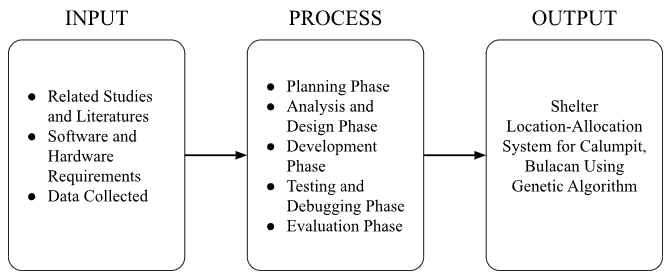
\includegraphics[width=\linewidth]{IPO}
		\label{IPOModel}
	\end{figure}
	
	The inputs for this project include related studies and literature, which provide a foundation for selecting and adapting an appropriate model for our system. These resources were analyzed and synthesized to establish a strong foundation in conducting this project. The researchers also needed to gather software and hardware requirements, such as compatible Windows versions and system prerequisites, to ensure a smooth development process. Additionally, real data from Calumpit, Bulacan, specifically community and shelter information, were essential for testing the system.
	
	The process begins with planning, where the researchers outline the objectives and approach for building the system. Once a clear plan is established, the researchers proceed to analysis and design, which involves creating mock-up designs, an ERD schema, and process flows to help developers visualize the system structure. Development phase is the longest phase, involving both frontend design and backend coding using the Qt framework. Once developed, the system has undergone rigorous testing to identify and correct any errors or anomalies, which are then debugged and resolved. Finally, the system was evaluated through a survey based on the ISO 25010 criteria to assess its acceptability.
	
	The expected output is a fully functional decision support system(DSS) that incorporates the  model adopted using a genetic algorithm as the solving method. The researchers generated results showing the optimal shelter location-allocation for Calumpit using the developed system.
	



\chapter{Research Methodology}

	This chapter outlines and expands upon the research methodology for the design and implementation of a shelter location-allocation system using a genetic algorithm for the optimization of shelter placement in disaster-prone areas. This methodology provides a systematic approach for a clear framework for system design, model implementation, and evaluation. Following this, data collection procedures are explained including the sources and techniques for gathering essential data on community demographics, geographic information, and shelter facilities.
	
	Additionally, this chapter addresses the criteria for selecting, cleaning, and analyzing data, as well as the metrics used to evaluate the system’s acceptability. Finally, ethical considerations such as data privacy are also discussed.

\section{Research Design}
	The research design for this study is mixed-method applied research, this approach combines both quantitative and qualitative methods to provide a structured framework for development and evaluation of the shelter location allocation system.

\subsection{Applied Research}
	The applied research aspect of this study focuses on developing and implementing a practical solution for shelter location-allocation in real-world scenarios. The primary objective is to create a shelter location-allocation system using a genetic algorithm.
	This applied research approach aims to deliver a functional and reliable shelter location-allocation system that local government units (LGUs) and disaster response agencies can easily deploy and adapt. By emphasizing incremental progress and user-centered development, this ensures that the research outputs are directly applicable and beneficial to communities in disaster-prone areas.

\subsection{Quantitative Research}
	The quantitative research component of this study aims to measure and analyze the acceptability of the proposing system using TAM determinants and ISO/IEC 25010 standard. The approach will provide objective and measurable evidence to evaluate the system's usability, reliability, and overall quality performance. The quantitative methods will seek to quantify the use of genetic algorithms in the shelter location allocation system, providing valuable insights into the system's effectiveness for emergency management.
	Methods will include collecting user feedback and performance metrics through structured surveys and system testing to assess these attributes. The survey will gauge user satisfaction with system usability and functionality using a 10-point rating scale, providing quantifiable insights into the system's ease of use and accessibility. 
	Incorporating quantitative research in this study is justified as it can provide empirical evidence supporting the shelter allocation system's acceptability. 

\subsection{Qualitative Research}
	The researchers will use qualitative research to understand the current issues of shelter location allocation from the stakeholders' perspectives. This approach requires engaging with the LGU offices to identify the additional requirements for the system. This ensures that the development of the shelter location-allocation system will address real-world challenges and support those involved in evacuating communities during natural disasters and be of acceptable quality.
	The researchers will conduct an interview to achieve this. The interview will be based on Decision Thinking Framework which is a common framework for developing a product. This was chosen to provide a structured way to gather detailed feedback from the stakeholders about their experiences, challenges, information about the shelters, and expectations regarding shelter location-allocation and this study. This method allows the researchers to collect various opinions and insights, which is important for understanding the complex issues involved in disaster management and shelter allocation.
	This insight is important for ensuring the system's effectiveness, as it helps identify the challenges to ensure the proper functioning of the shelter location allocation system and meet the needs of the affected communities. By capturing these detailed perspectives, the system will be more practical, user-friendly, and responsive to the real-world needs of disaster management.

\section{Model Adoption}
	The model adopted for this study is the Bilevel No-transfer (BNT) Model, which solves the shelter location-allocation problem under disaster scenarios. As discussed in a published paper by \textcite{LeahUP}, this model is effective when it assigns communities to shelters without allowing transfers between different shelter levels during recovery. Using the BNT Model, the researchers can optimize the allocation of communities to shelters, accounting for each shelter’s capacity and travel distance for evacuees.
	The BNT Model includes a two-tiered shelter structure, consisting of level 1 and 2 shelters. Level 1 shelters are smaller facilities intended for immediate use, providing basic services for short-term stays. In contrast, Level 2 shelters are significantly larger and equipped with comprehensive services, including private rooms and extended support amenities, these shelters are intended for longer-term stays. However, once assigned to a shelter in the BNT Model, evacuees remain in that shelter until the disaster subsides, eliminating the need for transfers between shelters.
	The objective function for the BNT model can be expressed as follows:
	
	Minimize 
	\begin{equation}
		wt_{dist}\sum_{j=1}^{N}\sum_{i=1}^{M}d_{ij}P_{i}x_{ij}+wt_{cost}\sum_{k=1}^{2}\sum_{j=1}^{N}C_{j}^{(k)}y_{j}^{(k)} 
	\end{equation}
	
	Subject to
	\begin{equation} 	
		\label{c1}
		d_{ij}x_{ij} \le D_{i}, \forall i = 1,..., M,  \forall j = 1,..., N 
	\end{equation}
	\begin{equation} 
		\label{c2}
		\sum_{i=1}^{M}LP_{i}x_{ij} \le \sum_{k} Area_{j}^{(k)} y_{j}^{(k)}, \forall j = 1,..., N , k=1,2
	\end{equation}
	\begin{equation} 
		\label{c3}
		\sum_{k=1}^{2} \sum_j={1}^{N}y_{j}^{(k)} \le MaxSh
	\end{equation}
	\begin{equation}
		\label{c4} 
		\sum_j={1}^{N}y_{j}^2 \le MaxL2
	\end{equation}
	\begin{equation}
		\label{c5}
		\sum_{j=1}^{N}x_{ij} = 1, \forall i=1,...,M
	\end{equation}
	\begin{equation}
		\label{c6}
		\sum_{k=1}^{N}y_{j}^{(k)} \le 1, \forall j=1,...,N
	\end{equation}
	\begin{equation}
		\label{c7}
	 	x_{ij}, y_{j}^{(1)},y_{j}^{(2)} \in \{0,1\}, \forall i=1,...,M,  \forall j=1,...,N
	\end{equation}
	
	Where:
	\\$wt_{dist}$ – weight given to the distance cost.
	\\$wt_{cost}$ – weight given to the fixed shelter cost.
	\\$M$ – total number of communities.
	\\$N$ – total number of potential shelter locations.
	\\$d_{ij}$ – distance between shelter i and community j.
	\\$P_{i}$ – population of the community i.
	\\$C_{j}^{(k)}$ – fixed cost for establishing shelter j of level k.
	\\$x_{ij}$ – binary decision variable indicating if community j is assigned to shelter i.
	\\$y_{j}^{(k)}$ – binary decision variable indicating if shelter j of level k is opened.
	\\$L$ - area allotted per individual
	\\$D_{i}$ – maximum distance that community i can be traveled.
	\\$Area_{j}^{(k)}$ - area of shelter j of level k.
	\\$MaxL2$ - maximum number of level 2 shelters to be opened.
	\\$MaxSh$ - maximum number of shelters to be opened.
	\\
	
	The constraints of BNT model include the distance, capacity, assignment, and binary constraints, each of which plays a crucial role in ensuring the model functions effectively under the disaster response scenario:
	
	\textit{Distance Constraint.} Equation \ref{c1} ensures that each community is allocated to a shelter within a defined maximum distance. 
	
	\textit{Capacity Constraint.} Equation \ref{c2} guarantees that the total number of evacuees assigned to a shelter does not exceed its maximum capacity. 
	
	\textit{Assignment Constraints.} Equations \ref{c3} and \ref{c4} ensures that the total assigned shelters and level 2 shelter does not exceeds over the user defined parameters respectively.  Equation \ref{c5} ensures that every community is assigned to exactly one shelter. Equation \ref{c6} ensures that the assigned shelter does not duplicate like being opened as level 1 and level 2 at the same time. This prevents problems in shelter allocation and ensures that each community has a designated place.
	
	\textit{Binary Constraint.} This constraint ensures that the model only takes binary variable, where can either be true (1) or false (0).
	
\subsection{Feasibility Conditions}

	Checking if a solution exists based on the user defined parameters is a must in developing the system thus conducting feasibility checks before executing the algorithm. This adds a feature that allows users to view if their inputs are incorrect having an additional functionality and capability of the system.
	
	The following conditions should satisfy else no solution exists:
	
	\begin{equation} 
		\label{f1}
		Area_{j}^{(2)} \ge Area_{j}^{(1)}, \forall j = 1, ..., N
	\end{equation}
	
	Condition \ref{f1} checks if shelter j area for level 2 is greater than or equal to their area for level 1. 
	
	\begin{equation} 
		\label{f2}
		MaxL2 \le MaxSh
	\end{equation}
	
	Condition \ref{f2} checks if the user defined number of maximum level 2 shelters is less than to number of maximum shelters.
	
	\begin{equation} 
		\label{f3}
		\exists j \in d_{ij} \le D_{i}, \forall i = 1, ..., M
	\end{equation}
	
	Condition \ref{f3} checks if there exists a distance from community i to all shelters that is less than or equal to its max distance.
	
	\begin{equation} 
		\label{f4}
		\exists i \in LP_{i} \le Area_{j}^{(2)}, \forall j = 1, ..., N
	\end{equation}
	
	Condition \ref{f4} checks if there exists a level 2 shelter that could accommodate a community i by their population multiplied by the area allotted per individual. 
	
	\begin{equation} 
		\label{f5}
		\sum_{i=1}^{M}P_{i} \le L\sum_{j=1}^{N}Area_{j}, \forall i=1,...,M,  \forall j=1,...,N
	\end{equation}
	
	Condition \ref{f5} checks if the total population is less than or equal to the total area of shelters multiplied to area allotted per individual. If this fails, then it is theoretically impossible to allocate all individuals given with their shorted capacity of shelters.
	
	Incorporating these feasibility conditions ensures that the model will produce atleast one feasible solution, and the system proceeds only with valid input configurations. By verifying these conditions, users receive instant feedback on whether their inputs are valid, allowing the model to proceed with solving. These conditions represent key feasibility checks but are not exhaustive, and infeasible solutions may still persist. An additional feature would employ a penalty function that would transform the model to an unconstrained model.	
	
\subsection{Penalty Function}
	The penalty function will be used to handle the problem constraints. Instead of discarding infeasible solutions or chromosomes, they will be assigned a very large objective value making them not fit to be a solution. The type of penalty to be used is the Courant-Beltrami penalty function method, as shown in equation \ref{p1}.
	
	\begin{equation} 
		\label{p1}
		h(x)=(g^+(x))^2
	\end{equation}
	
	where
	
	\begin{equation} 
		\label{p2}
		g^+(x)=max\{g(x),0\}
	\end{equation}
	
	where $g(x)$ is a constraint function of the form $g(x)\le0$. 
	\\
	The new objective function would be adding the initial objective value $f(x)$ to the penalty multiplied by some constant $\gamma$ as shown in equation \ref{p3}.
	
	\begin{equation} 
		\label{p3}
		f_(new)(x)=f(x)+\gamma\sum_{i=1}^{n}(max\{g_i(x),0\})^2
	\end{equation}
	
	where $g_1(x),g_2(x),...g_n(x)$ are the constraints of the model of the form $g_i(x)\le0$, and $\gamma\in\mathbb{R}^+$ is sufficiently large. The penalty would add up to the objective value for each constraints it violated, otherwise it would not affect the objective value.	
	
\subsection{Optimization Technique}
	In a study created by \textcite{Mathew2012}, Genetic Algorithms are based on the concept of natural selection and evolves possible solutions through operators such as selection, crossover, and mutation. This algorithm will iteratively evolve a population of potential solutions, utilizing operations to explore the population space and gradually converge toward an optimal solution.
	
	The BNT model was originally solved using Binary Genetic Algorithm implemented in MATLAB. However, since system integration will be conducted on this thesis, the model will be solved using Integer-based Genetic Algorithm implemented in Python. This decision derived for satisfying the assignment constraint of the model, and Python being a well suited programming language for both data simulation and system development.
	
	We start by defining the some terms of genetic algorithm that will be used in the context of shelter location-allocation model.
	
	\textit{Chromosome.}  An array or dictionary which represents the  solution in a problem. A chromosome is composed of two parts, community allocation and shelter level. Community allocation refers to assigning shelter index to communities, and shelter level refers to assigning a value of 1 or 2 to represent as level to shelters. Figure \ref{Chromosome} shows a solution where community 0 was allocated to shelter 0, and community 1 and 2 was allocated to shelter 1. Additionaly, shelter 0 was assigned as level 1, and shelter 1 was assigned as level 2.
	
	\begin{figure}[h!]
		\caption{A chromosome with 3 communities and 2 shelters}
		\centering
		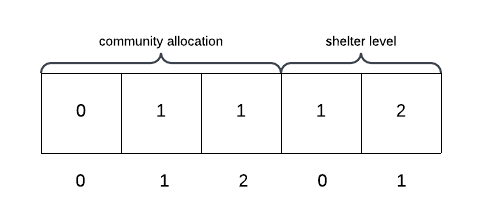
\includegraphics[width=250px]{Chromosome}
		\label{Chromosome}
	\end{figure}
	
	\textit{Population.} A group of chromosomes. This refers to a group of generated solutions on the problem that will be later on picked or selected.
	
	\textit{Generation.} A whole iteration process of genetic algorithm. This refers to the population on a certain generation which in theory, higher generations then the closer we get to the optimal solution.
	
	\textit{Fitness.} A value generated from the objective function. This refers to the objective value of a chromosome based on the implemented model.
	
	A genetic algorithm is composed of three key components: selection, crossover, and mutation. Each serves a distinct purpose in addressing optimization problems and simulates the evolution theory. Each component has various implementation methods tailored to specific objectives. \parencite{Eyal2020}
	
	\textit{Selection.} A process of selecting parents. This refers to selecting two chromosome based on their fitness value. The proposed system uses Roulette Wheel Selection, which is the likelihood of a chromosome to be selected is directly proportional to its fitness value. Figure \ref{Selection} shows that the probability is inversely proportional to the fitness value, since we aim to minimize the objective. Moreover, a randomizer will select a chromosome based on the computed probabilities.
	
	\begin{figure}[h!]
		\caption{Selection process where probability is based on their fitness value.}
		\centering
		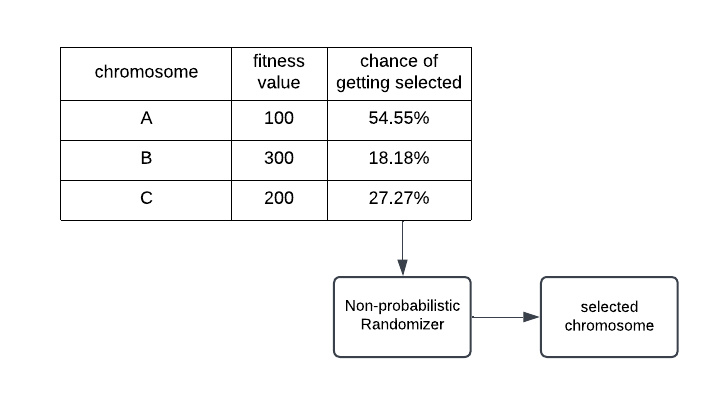
\includegraphics[width=350px]{Selection}
		\label{Selection}
	\end{figure}
	
	\textit{Crossover.} A process of breeding and giving offspring by a two parents. This refers to combining two selected chromosome values and generating a new chromosome based on the combined values. The proposed system uses Uniform Crossover, which all the values from two parents has a change to be inherited by the offspring. Figure \ref{Crossover} shows a generated offspring with values based on their parents. Notice that if a value is different between parents, a randomizer will decide which value would be chosen.
	
	\begin{figure}[h!]
		\caption{Crossover process where parents generate a new offspring}
		\centering
		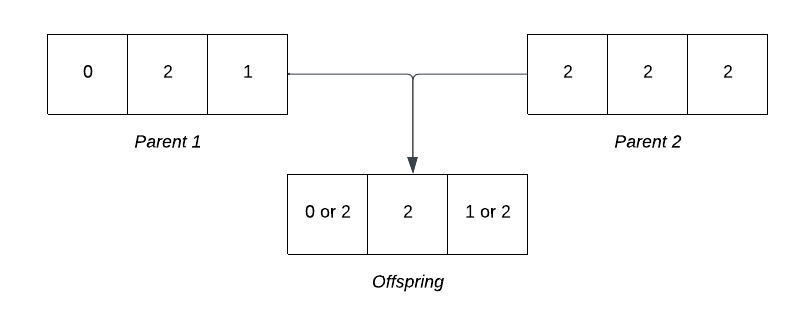
\includegraphics[width=350px]{Crossover}
		\label{Crossover}
	\end{figure}
	
	\textit{Mutation.} A process of altering some chromosome values. This refers to randomly selecting a chromosome from a population based on a predetermined mutation rate, then changing some of its values. The proposed system uses Random Reset Mutation, which picks randomly from a selected chromosome values, then changing it by generating a new random number. Figure \ref{Mutation} shows altering of a chromosome for the second community by a randomizer, allocating from shelter 1 to shelter 2.
	
	\begin{figure}[h!]
		\caption{Mutation process where a value is randomly altered}
		\centering
		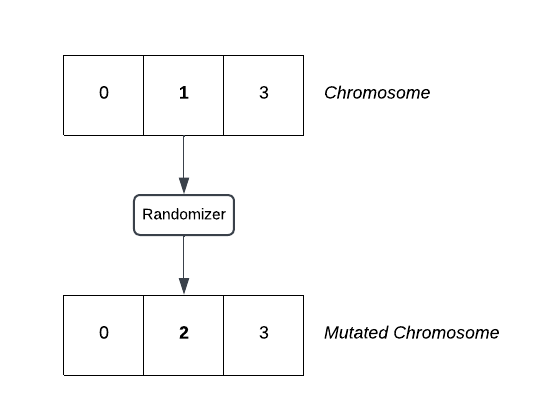
\includegraphics[width=300px]{Mutation}
		\label{Mutation}
	\end{figure}
	
	By applying these evolutionary principles, the genetic algorithm can efficiently navigate the large and complex problem space of shelter allocation, ensuring the most effective distribution of evacuees to shelters based on the model’s constraints and objectives.
	

	
	
\section{Process of Developing the System}
	This study employs a structured system development methodology following the Agile approach. Agile was chosen for its flexibility and iterative nature, which allows for continuous refinement and adaptation of the system based on feedback and testing results. Each development phase—planning, design, implementation, testing, and deployment—will include regular reviews and adjustments to ensure the system evolves effectively to meet technical and user needs.
	The system development process is divided into several distinct phases, each of which is designed to build upon the previous stage, ensuring a comprehensive and systematic approach. As shown in figure \ref{Agile} illustrated by \textcite{Jayathilaka2020}

	\begin{figure}[h!]
		\caption{A representation of an Agile approach}
		\centering
		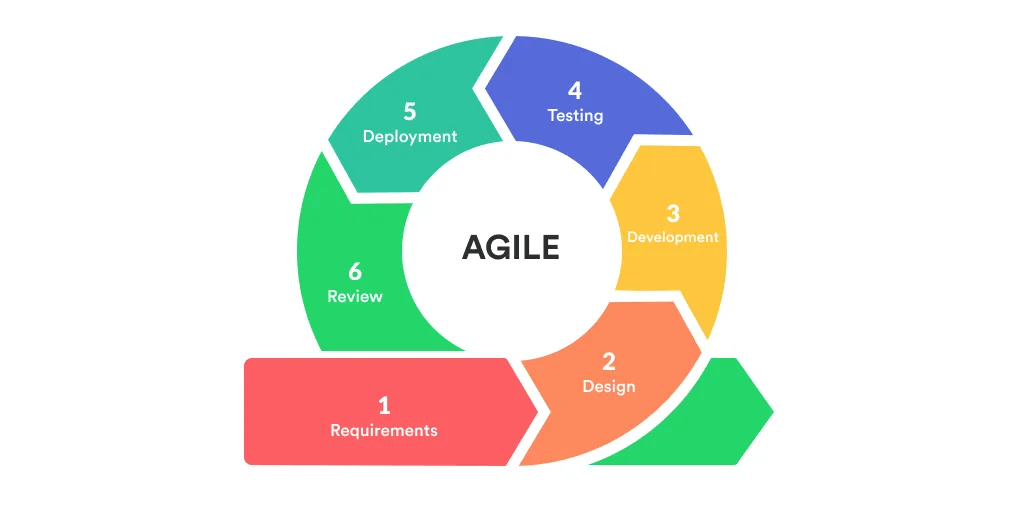
\includegraphics[width=\textwidth]{AGILE}
		\label{Agile}
	\end{figure}

\subsection{Planning}

	In the initial phase, the researchers outlined the shelter location allocation system's scope, objectives, and requirements. This process identifies the key features and functionalities essential for the system. Additionally, this phase includes the thesis project plan, which details the project timeline.
	The Gantt chart outlines the phases of the thesis project, including thesis one output, thesis two output, data collection and preparation, paper miscellaneous, system design, system development, and system assessment. Each phase addresses specific objectives that contribute to completing the shelter location-allocation system. The Gantt chart is shown in Figure \ref{Gantt}.
	
	\begin{landscape}
		\begin{figure}[h!]
			\caption{The Gantt Chart}
			\centering
			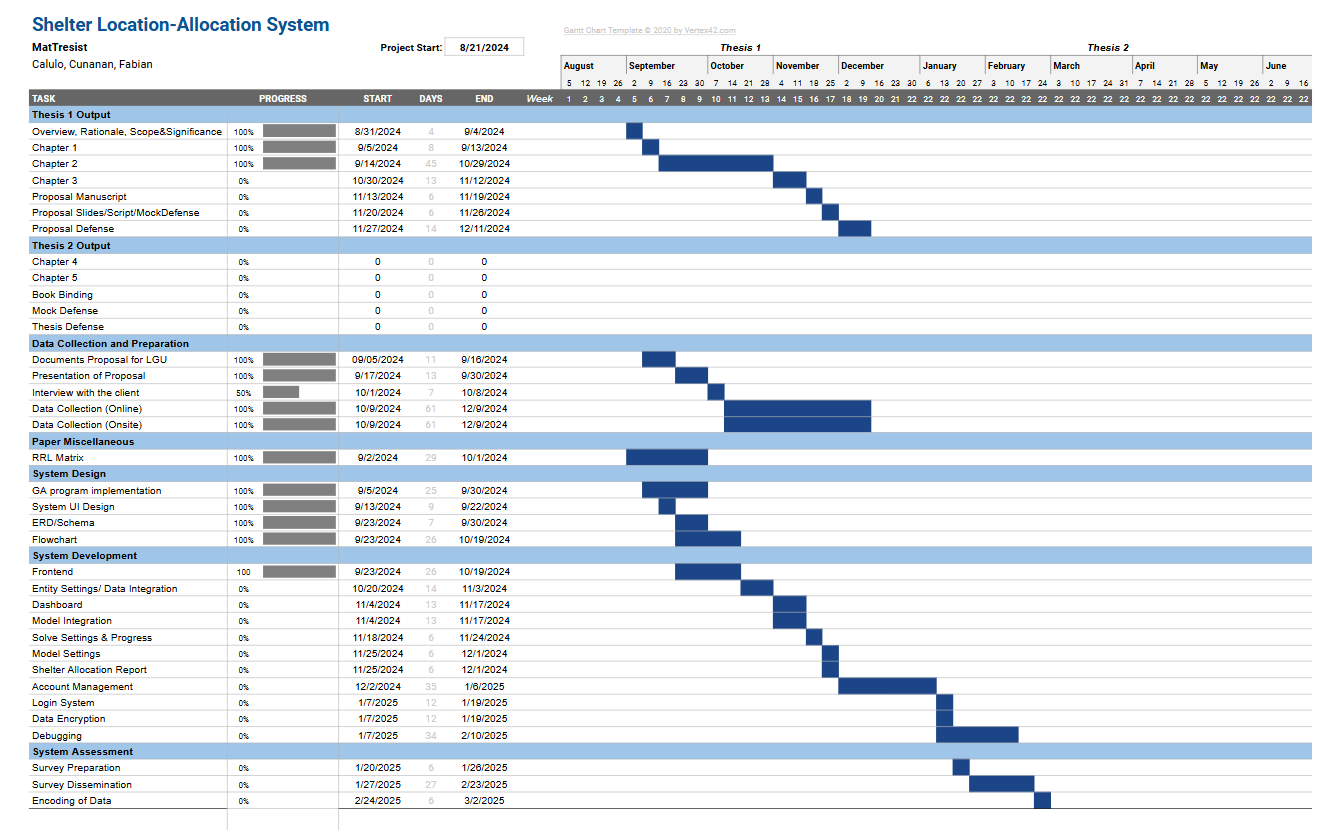
\includegraphics[width=600px]{Gantt}
			\label{Gantt}
		\end{figure}
	\end{landscape}
	
	\textbf{Thesis One Output:} This phase involves drafting the initial sections of the thesis, such as the overview, rationale, scope, and significance, along with Chapters one through three (Introduction, Review of Related Literature, and Methodology). Additionally, this phase includes preparing the proposal manuscript, slides, and script for the mock defense and proposal defense. Parallel to this is the Paper Miscellaneous, which includes the creation of the literature review matrix to organize and support the contents of Chapter 2. This approach maintains a well-structured reference base for literature review.
	
	\textbf{Thesis Two Output:} Following the foundational work in the first thesis phase, this continues the development of this thesis document, focusing on Chapters 4 and 5 (Results and Conclusions) and preparing for the mock defense and final thesis defense. This phase signifies the completion of the thesis writing process.
	
	\textbf{Data Collection and Preparation:} This critical phase entails gathering data required for system design and important data for the genetic algorithm. Tasks include submitting documents to the LGU, presenting the project proposal, conducting client interviews, and collecting online and onsite data.
	
	\textbf{System Design:} This phase focuses on planning the technical aspects of the shelter allocation system, including genetic algorithm implementation, user interface design, entity relationship diagram, and flowchart development. These elements form the blueprint that guides the system's development.
	
	\textbf{System Development:} The project's core phase involves the actual construction and coding of the system. Tasks include front-end development, data and model integration, dashboard creation, and implementing security features. This phase also includes testing and debugging to ensure system functionality.
	
	\textbf{System Assessment:} The final phase, along with Thesis Two Output, is evaluating the system's acceptability and user satisfaction. Activities include preparing and distributing surveys, gathering user feedback, encoding and analyzing this data to assess system acceptability.

\subsection{Requirement Analysis}
	During the requirement analysis phase, researchers gather comprehensive information about the system requirements by reviewing relevant literature that pertains to the thesis. Moreover, an interview with the client is conducted to know more about the current issues LGUs are facing regarding to evacuation. This phase ensures that all necessary features are identified and prioritized based on their importance.
	
	The system's primary features and requirements encompass an overview of data and model modification, data simulation, shelter tagging, and report encryption. Data modification includes an access to user for managing and modifying community and shelter data. Model modification allows users to change parameters on data simulation.Data simulation utilizes the community and shelter data as inputs for the genetic algorithm applied in the shelter location allocation system, optimizing the placement of evacuees in shelters. Furthermore, shelter tagging enables the categorization of shelters based on criteria such as location, capacity, and suitability for various disaster scenarios, thereby facilitating efficient resource allocation. Lastly, report encryption allows user to encrypt their generated report to prevent leaks in a computer system.
	
\subsection{Design}
	During the design phase, the researchers created a detailed outline for the shelter location-allocation system's architecture and key components. The design process includes creating a mockup of the system's user interface and constructing flowcharts, an entity-relationship diagram (ERD), and a data flow diagram(DFD) to map out system processes and data relationships. The researchers designed mockups to visualize the user interface, ensuring it met the user's needs for accessibility and usability. The flowcharts provided a step-by-step breakdown of system processes, while the ERD defined the data structures and relationships. These elements formed a cohesive blueprint to guide the system's development and ensure alignment with the requirements. Figure \ref{SystemArch} shows the system architecture which combines DFD and the interaction of users.

	\begin{figure}[h!]
		\caption{System Architecture}
		\centering
		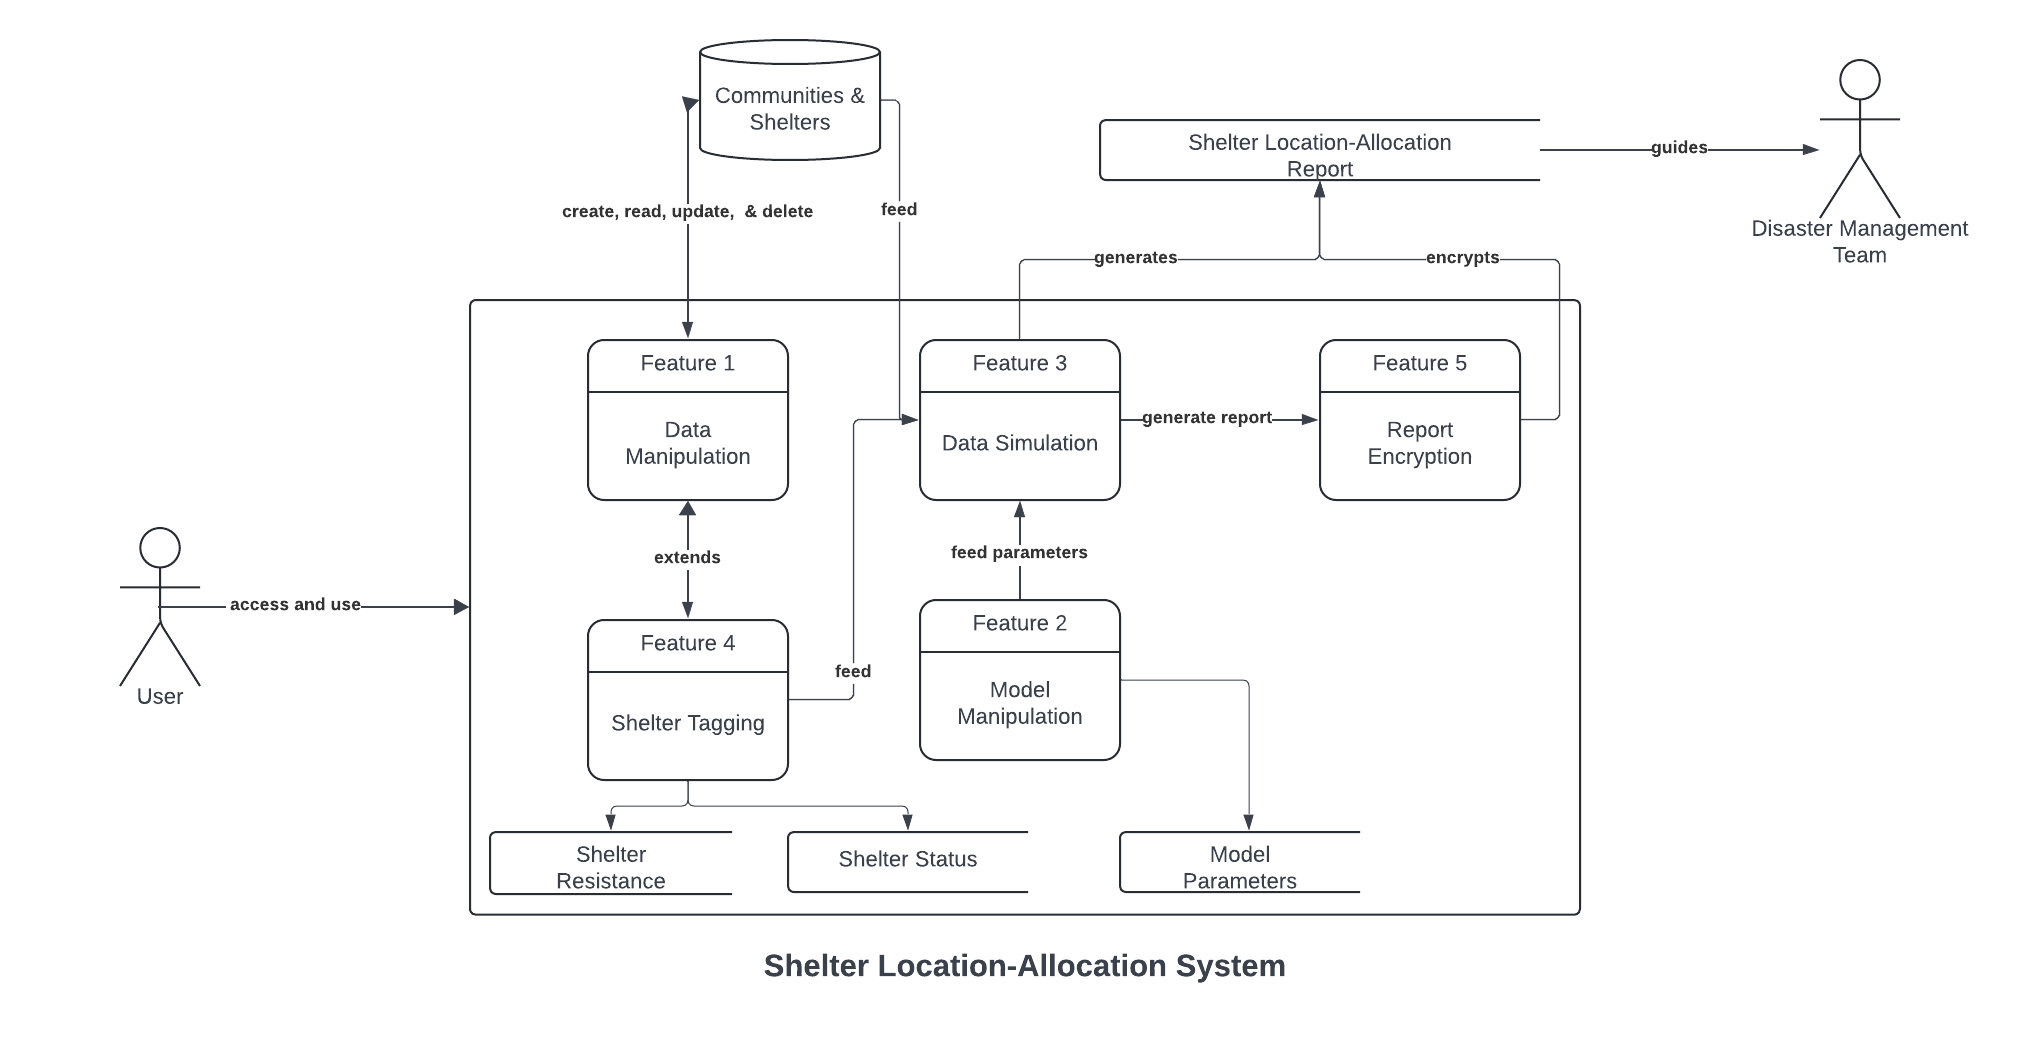
\includegraphics[width=\textwidth]{Context Diagram}
		\label{SystemArch}
	\end{figure}
	
	The system architecture involves the interaction of two actors, the user of the system and disaster management team. The community and shelter data will be fed into a system which features data manipulation and shelter tagging. With the cleaned or finished data, data simulation may begin together with the model parameters modified by the user. Finally, a report will be generated and can be encrypted or not. The report will be used by the disaster management team to guide them for decision making in allocation of residents to the correct shelter.

	\begin{figure}[h!]
		\caption{The ERD Schema}
		\centering
		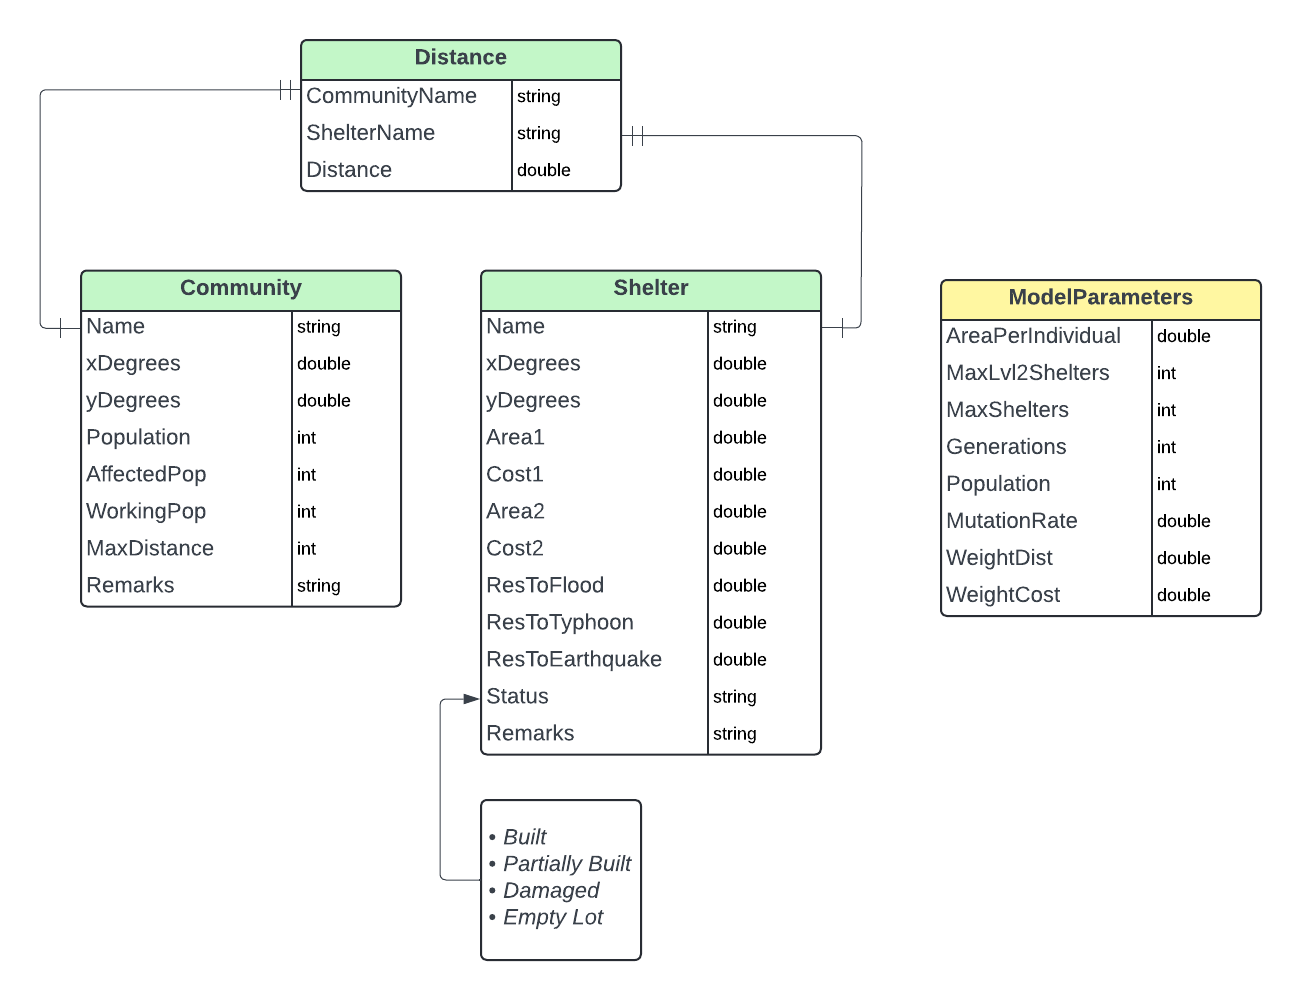
\includegraphics[width=\textwidth]{ERD}
		\label{ERD}
	\end{figure}
	
	Figure \ref{ERD} shows the entity relationship (ERD) which has 4 entities: Community, Shelter, Distance, and ModelParameters. Distances are derived from the location of Shelter and Community, then will be saved accordingly to be used in performing the system model. ModelParameters shows no relationship since it only saves the current settings for the model and algorithm.
	
	\begin{figure}[h!]
		\caption{Overview of System Mock-up}
		\centering
		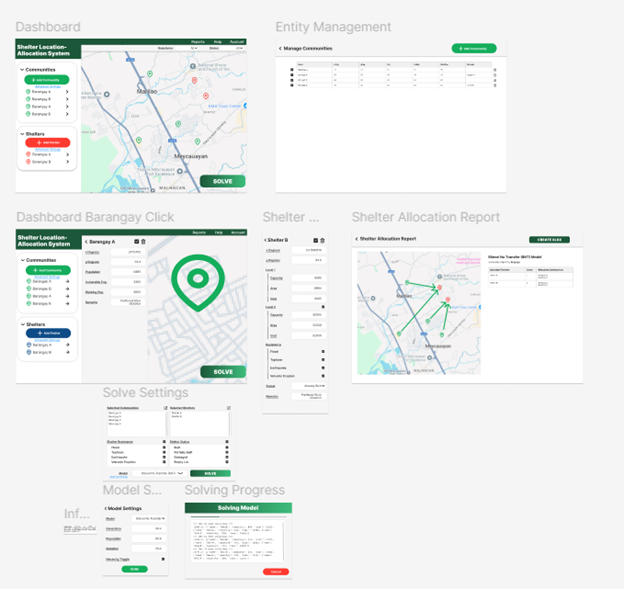
\includegraphics[width=\textwidth]{SYSTEM MOCKUP}
		\label{Mockup}
	\end{figure}
	
	As can be seen in Figure \ref{Mockup}, The system mock-up shows the prototype of the system by designing the User Interface (UI) using a prototyping tool, Figma. This shows the UI for different modules of the system: Dashboard, Entity Management, Shelter Allocation Report, Settings, and the Progress.

\subsection{Development}
	The development phase will include coding and implementing the genetic algorithm for the shelter location allocation system. Utilizing the Agile system development life cycle, which includes weekly meetings and development reviews, the team can ensure that development remains on track and that any issues are promptly addressed. By following the Agile SDLC, the researchers can adapt quickly to any changes in requirements, maintain clear communication, and address any issues promptly.
	
	Table \ref{TechUsed} shows the list needed to start the development process. The system will be developed using Python programming language, and Qt framework to efficiently implement the graphical user interface(GUI) of the system. Visual Studio Code will be utilized as the integrated development environment (IDE), and QtDesigner as an extension for creating frontend designs by Qt framework.
	
	\begin{table}[h]
		\centering
		\caption{List of tools and technologies used in the development process}
		\label{TechUsed}
		\resizebox{\textwidth}{!}{
			\begin{tabular}{|c|c|p{8cm}|}
				\hline
				\multicolumn{1}{|c|}{\textbf{Name}} & 
				\multicolumn{1}{c|}{\textbf{Version}} & 
				\multicolumn{1}{c|}{\textbf{Description}} \\ \hline
				Visual Studio Code   & 1.96.3   & IDE for the whole coding and debugging process            \\ \hline
				Python               & 3.12.5   & Programming language known for extensive computation libraries  \\ \hline
				QtDesigner           & 5.11.1   & GUI design tool which has drag and drop feature \\ \hline
				GitKraken            & 10.6.1   & Git client that is user friendly for executing Git commands      \\ \hline
				GitHub               & Web      & Repository host which used for collaboration and backup of the project\\ \hline
			\end{tabular}
		}
	\end{table}
	
	Developing the proposed system using Python allows us to use Python libraries. As shown in Table \ref{PythonUsed}, displays all the libraries used to develop the system. PySide6 is responsible for the GUI that uses the Qt framework. Pandas and openpyxl are used for handling data. Folium, OSMnx, networkx, and scikit-learn are for displaying and calculating the map shown in the system. Lastly, numpy is used for executing genetic algorithm.
	
	\begin{table}[h]
		\centering
		\caption{List of libraries installed in Python}
		\label{PythonUsed}
		\resizebox{\textwidth}{!}{
			\begin{tabular}{|c|c|p{8cm}|}
				\hline
				\multicolumn{1}{|c|}{\textbf{Name}} & 
				\multicolumn{1}{c|}{\textbf{Version}} & 
				\multicolumn{1}{c|}{\textbf{Description}} \\ \hline
				PySide6   & 6.7.2   & Uses Qt framework for frontend development \\ \hline
				pandas               & 2.2.3   & Reads and handles datasets  \\ \hline
				openpyxl            & 3.1.5   & Opens and reads excel files \\ \hline
				folium            & 0.17.0   & Provides visualization and interactivity on a geographical map  \\ \hline
				osmnx               & 1.9.4      & Retrieves OpenStreetMap(OSM) data and could calculate road paths\\ \hline
				networkx               & 3.3      & Creates and computes complex graphs such as road networks\\ \hline
				scikit-learn               & 1.5.2      & Provides simple machine learning tools and functions\\ \hline
				numpy               & 1.26.4     & Generates non probabilistic numbers \\ \hline
				msoffcrypto-tool & 5.4.2     & Encrypts and decrypts excel files \\ \hline
				XlsxWriter & 3.2.2     & Edits and writes excel contents \\ \hline
				
			\end{tabular}
		}
	\end{table}
	
	
	
\subsection{Testing and Debugging}
	The system will undergo functionality, performance, and reliability testing during the testing phase. The researchers will employ manual testing techniques to identify and resolve any bugs or issues that arise. Found any errors and anomalies within the system, it will be then fixed and debugged. Through this thorough testing and debugging approach, the researchers aim to ensure that the shelter location allocation system meets high quality, performance, and user satisfaction standards, making it ready for deployment.
	
\subsection{Deployment}
	During the deployment phase, the shelter location-allocation system will undergo pilot testing in collaboration with local government units (LGUs). This process will involve configuring the system, establishing the necessary data inputs, and training users to utilize the platform effectively. Additionally, the deployment phase will continuously monitor the system's performance to ensure it operates efficiently and meets the objective of optimizing shelter locations. 

	\textbf{Sustainability Plan}
	The presentation of the application to the potential users, specifically the Local Government Unit (LGU) of Calumpit will include a walkthrough tutorial covering all essential features. The users will be provided with the information necessary to operate the app effectively, including an overview of its purpose, functionalities, and how to input relevant data. Specifically, this includes entering shelter locations, population data, and accessibility metrics into the system to ensure accurate allocation results. Since a detailed explanation was provided during the system evaluation, this presentation will focus on summarizing key points and addressing questions and feedback from the users.

	Feedback gathered from the potential users will be important in identifying the areas for improvement. This feedback will be collected through structured surveys and interviews to provide a comprehensive understanding of user needs and challenges. The updates and adjustments to the application from the feedback to better align the users’ needs, the new version of the application will be emailed to the Local Government Unit (LGU) of Calumpit for operational use. This will ensure that they have access to the latest features and improvements. It is important to note that this application is copyrighted by Bulacan State University to protect its intellectual property and ensure proper recognition to the researchers, developers, and thesis adviser. This copyright also prevents unauthorized commercial use and distribution, ensuring that the application remains a free resource for its intended purpose. It is not for sale.
	
\subsection{Evaluation}
	Evaluation of system includes preparing ang distributing survey questionnaires based on TAM and ISO/IEC 25010 to our target sample. This phase will ensure that the developed system has feedback from potential users as well as from experts in software engineering and development.

\section{System Preliminaries}
	Developing a system requires careful planning and analysis before implementing it. A communication between the potential users or clients and the researchers is essential to ensure all system requirements are met and improved. This phase aims to establish a foundational understanding of current disaster-response processes, along with gathering essential data for the system. Interviews will be conducted with representatives from local government units (LGUs) specifically from the target population to understand their existing shelter allocation process, challenges, and expectations for a decision support system. 
	
\subsection{Client Interview}
	Conducting an interview with the client is essential to get to know with the potential users and the problems their facing. Questions formulated are derived from Design Thinking Framework which is according to \textcite{Julio2018} has resulted a greater approximation of end users and the development team who uses an Agile SDLC. This improves the quality and usability of the software.
	
\subsection{Data Gathering}
	The model needed data to perform, specifically community and shelter data. Additionally, to ensure that the system produces outputs, data on shelters, disaster events, and typhoons will be collected. This includes accessing records on past typhoon impacts, available shelter locations, and their respective capacities. Community or barangay data will be sourced from publicly available databases, such as PhilAtlas, which provides detailed geographical and demographic information essential for accurate system modeling.
	
\subsection{Data Preprocessing}
	Once data collection is complete, the gathered information will undergo several stages: cleaning, processing, analysis, and interpretation. This ensures it meets the needs of the system and allows for an accurate assessment of its effectiveness.
	
	All collected data will first be cleaned to remove any inconsistencies, duplicates, or irrelevant information. This process is crucial for ensuring the data’s quality and reliability, particularly for a system that relies on precision in both inputs and outputs. Any insufficient data will be asked on the LGU to fill in the gaps of the datasets. 
	
	The table \ref{dataSource} presents all the data variables on communities and shelters used in the model, along with their respective sources. Improvement or rehabilitation cost is added for costs which are based on a report for improvement of an evacuation center from DILG, which cost approximately ₱7,700 per square meter. Meanwhile, data for Level 2 shelters are simulated, as the LGU does not have a data nor system for the hierarchy of shelters. The areas are assumed to be twice their initial size, and costs are estimated based on the contract cost of the Frances Evacuation Center, as detailed in the DILG and DPWH reports, resulting in approximately ₱60,000 per square meter.
	
	\begin{table}[h]
		\centering
		\caption{Variables, Descriptions, and Sources for Community and Shelter Data}
		\label{varDescriptionSource}
		\resizebox{\textwidth}{!}{
			\begin{tabular}{|c|c|p{8cm}|}
				\hline
				\textbf{Variable} & \textbf{Source} & \textbf{Description} \\ \hline
				\multicolumn{3}{|c|}{\textit{\textbf{Community}}}\\ \hline
				Name & LGU interview & Identity of a community \\ \hline
				Longitude & Google Map \& LGU interview & Longitudinal coordinates \\ \hline
				Latitude & Google Map \& LGU interview & Latitudinal coordinates \\ \hline
				Population & Philippine Atlas (2020 population) & Number of individuals living in a community \\ \hline
				AffectedPop & LGU interview (from Typhoon Karina 2024) & Number of individuals affected during a disaster \\ \hline
				MaxDistance & Maximum distance generated in distance calculation & Distance allowed to travel by a community \\ \hline
				\multicolumn{3}{|c|}{\textit{\textbf{Shelter}}} \\ \hline
				Name & LGU interview & Identity of a shelter \\ \hline
				Longitude & Google Map \& LGU interview & Longitudinal coordinates \\ \hline
				Latitude & Google Map \& LGU interview & Latitudinal coordinates \\ \hline
				Area1 & Google Map & Lot area of a shelter (level 1) \\ \hline
				Cost1 & Assumed 7,700 * Area1 & Cost for constructing/maintaining a shelter with Area1 \\ \hline
				Area2 & Assumed Area1 * 2 & Lot area of a shelter (level 2) \\ \hline
				Cost2 & Assumed 60,000 * Area1 & Cost for constructing/maintaining a shelter with Area2 \\ \hline
				ResToFlood & LGU interview & Is the shelter resistant to flood? \\ \hline
				ResToTyphoon & LGU interview & Is the shelter resistant to typhoon? \\ \hline
				ResToEarthquake & LGU interview & Is the shelter resistant to earthquake? \\ \hline
				Status & LGU interview & State of the physical structure of a shelter \\ \hline
				\multicolumn{3}{|c|}{\textit{\textbf{Distance between Community and Shelter}}} \\ \hline
				distance & OpenStreetMap API & distance needed to travel by a community to a shelter  \\ \hline
			\end{tabular}
			}
	\end{table}
	
	Researches added empty lots across Calumpit to be appended to shelter data. These lots are identified and selected to be resistant to hazards, specifically floods with the assistance of Nationwide Operational Assessment of Hazards (NOAH) website. Table \ref{AppendData} shows the change of variables in area, cost, resistance and status for these appended shelter data. Additional cost is added due to property cost which according to Dot Property, approximately ₱12,500 per square meter was the average cost for land in Calumpit.
	
	\begin{table}[h]
		\centering
		\caption{Sources of Appended Shelter Data}
		\label{AppendData}
			\begin{tabular}{|c|c|}
				\hline
				\multicolumn{1}{|c|}{\textbf{Variable}} & 
				\multicolumn{1}{c|}{\textbf{Source}} \\ \hline
				Cost1     & Assumed Area1 * (60,000 + 12,500) \\ \hline
				Cost2     & Assumed (Area2 * 60,000) + (Area1 * 12,500) \\ \hline
				ResToFlood     & Assumed TRUE \\ \hline
				ResToTyphoon    & Assumed TRUE \\ \hline
				ResToEarthquake     & Assumed TRUE \\ \hline
				Status     & Already an Empty Lot \\ \hline
				
			\end{tabular}
	\end{table}
	
	For justification of the target area’s vulnerability, typhoon data spanning from 2006 to 2022 will be examined. This dataset includes the number of affected and evacuated individuals across various municipalities in Bulacan. The data will be grouped by municipality, summing the affected and evacuated residents over the specified period. This analysis helps justify the focus on the municipality and supports the rationale for the shelter allocation model’s implementation in the municipality.
	
	The cleaned shelter and community data will be fed into the system to facilitate accurate shelter location-allocation modeling. The system will use these inputs to generate optimized shelter placement recommendations based on the model adopted.
	
	
\section{System Evaluation}
	System evaluation will focus on assessing acceptability of the shelter location allocation system using the TAM determinants and ISO/IEC 25010 standard. These standards provides a framework for evaluating the software's quality and acceptability. The system evaluation will include the evaluation instrument, determining the population and sample, outlining data collection procedures, and discussing the data analysis techniques used.

\subsection{Evaluation Instrument}
	The evaluation instrument is a structured questionnaire designed to assess the acceptability of the shelter location allocation system based on the determinants of Technology Acceptance Model(TAM) and key quality attributes outlined in the International Organization for Standardization and International Electoral Commission (ISO/IEC) 25010 standard. Questionnaires based on TAM will be distributed to the potential end-users of the system. On the other hand, questionnaires based on ISO/IEC 25010 will be distributed to the experts in software development.
	
	TAM questionnaire will evaluate the system's acceptability by the user of the system. This model answers why users accept or reject information systems, and examines a system's acceptance based on their attitudes, preferences, and behaviors.\parencite{Davis1987}
	\\The following criteria are based upon the four determinants defined in TAM:
	
	\textit{Perceived Usefulness.} This answers on how much a user believes using the system will improve their performance such as job tasks. It evaluates whether the users thinks the proposed system will be genuinely beneficial to LGUs or if it can assist other LGUs effectively.
	
	\textit{Perceived Ease of Use.} This answers on how much a user believes using the system will be efficient and user-friendly. It considers whether the proposed system can be used smoothly with minimal errors and without performance issues.
	
	\textit{Attitude Towards Using.} This answers on what user feels when using the system based on their enjoyment and satisfaction. A positive attitude towards the system often leads to accepting the technology.
	
	\textit{Behavioral Intention to Use.} This answers on willingness to use the system in the future. It determines whether users find the system valuable enough to incorporate into their long-term plans.
	
	Additionally, ISO/IEC 25010 questionnaire will evaluate various aspects of the system, including usability, reliability, performance efficiency, and overall user satisfaction. Through this instrument, the study aims to gather objective data that will help determine how well the system meets user needs and expectations. \parencite{ISOIEC2023}
	\\The following criteria are based upon the nine quality characteristics for product quality model defined in ISO/IEC 25010:
	
	\textit{Functional Suitability.} This evaluates how well the system meets user needs and performs its intended functions. The questions will focus on the system's ability to allocate shelters effectively, manage community and shelter information, and provide accurate data.
	
	\textit{Performance Efficiency.} This attribute will evaluate the system's response time and processing capacity. The questionnaire will include items assessing the system's speed in performing functions, efficient use of resources such as memory and processing power, and ability to handle maximum load requirements. By examining performance efficiency, the study aims to determine whether the system can perform reliably under diverse operational conditions.
	
	\textit{Compatibility.} This will assess the system’s ability to exchange and use information with other systems. The questionnaire will ask how well the system integrates with external databases, applications, or computer systems. 
	
	\textit{Interaction Capability.} This will prioritize the system's usability, learnability, and overall user satisfaction. The questionnaire will gather detailed user feedback regarding their experiences with the system. The questionnaire will address aspects such as ease of navigation, effectiveness in completing tasks, and general user engagement.
	
	\textit{Reliability.} This attribute will assess the system's interaction capability, focusing on its ease of use, appropriateness for users, and ability to guide users in completing tasks effectively. The evaluation will include questions on how easily users can recognize if the system meets their needs, learn its functions, and operate it with minimal errors. Additional focus will be on user engagement, inclusivity, and the availability of assistance to support a diverse range of users. 
	
	\textit{Security.} The system ensures that all collected data will remain confidential and solely for this research. No data will be uploaded online, and all information will be stored offline. Access to data will be limited to the researchers and users.
	
	\textit{Maintainability.} This will evaluate the system's ease of adaptability to meet new requirements, correct errors, and improve performance. The questionnaire will assess the system's reusability, analyzing how parts of the system can be leveraged in future developments or other systems, and its testability, ensuring that any necessary changes can be efficiently implemented and quickly identified so that testing can be done efficiently. 
	
	\textit{Flexibility.} This will assess the system’s ability to adapt to changing user needs and requirements. The questionnaire will evaluate the system's ability to support new features, incorporate updates, and seamlessly integrate with additional tools or systems as necessary. It will also examine how well the system accommodates changes in shelter allocation criteria, such as shifts in population density and shelter resistance.
	
	\textit{Safety.} This will evaluate the system's ability ensures it does not expose any potential harm to the users and communities. The questionnaire will assess whether the shelter allocation outputs prioritize safe locations, avoiding disaster-prone areas such as flood zones, landslide-prone areas, or unsafe structures. This includes also evaluating the accuracy of the system's data to prevent errors that might jeopardize users.

\subsection{Population and Sample}
	The population of this study will consist of end-users and IT experts. For end-users,  MDRRMO and MSWDO of the municipality of Calumpit. Meanwhile for IT experts, includes CICT professors from Bulacan State University, and someone who have experience in developing a system.  The diversity of perspective of these are important for the comprehensive evaluation of the system’s acceptability.
	
	\textbf{MDRRMO:} The staff consists of Municipal Disaster Risk Reduction Management Office, who are responsible for formulating and implementing the province's disaster risk reduction plan.  Their insights are vital for understanding the operational requirements considerations for implementing the shelter location allocation system, ensuring it aligns with established disaster response protocols and local needs.
	
	\textbf{MSWDO:} The Municipal Social Welfare and Development Office plays a key role in managing the evacuation and welfare of the communities during disasters. Their expertise is essential in ensuring that the shelter allocation system aligns with evacuees' specific needs, such as accessibility and capacity to the shelter location allocation across the province. Their input will help tailor the system to address the welfare requirements of evacuee management during emergencies.
	
	\textbf{CICT professors:} Coming from the College of Information and Communication Technology, professors have significant academic background and experience to technologies. This part of population will assess the system's performance and functionality with the help of their knowledge and expertise.
	
	\textbf{System Developers:} Experts with extensive experience in system development play an important role in project evaluation. They are commonly found in businesses that design, propose, and develop systems for their clients. Their expertise enables them to understand and address real-world client requirements, guiding the system to be acceptable to users.
	
	The sampling technique that will be utilized for end-users is Stratified Sampling Technique, where the population is divided into a respective groups or strata, where in this study, our stratum is the MDRRMO and MSWDO. This ensures comprehensive representation, to capture the perspectives of different stakeholder groups proportionately. The sample size of end-users will be computed using G*Power, a statistical software tool. With a confidence level of 95\% or 0.05 margin of error, the sample size would be 23. Since the sample size would be much smaller than the population size, then conducting system evaluation would be feasible.
	
	Meanwhile, for IT experts, Purposive Sampling Technique will be employed. Researchers will purposively select 10 IT experts from CICT who have experience in system development or have worked in a government agency related to disaster risk management. These experts will be chosen based on their qualifications and relevant experience to provide insights into the system's design, functionality, and performance. This technique ensures that the selected experts evaluating the system will provide comprehensible and accurate feedback while also ensuring its feasibility.
	
\subsection{Data Collection Procedures}
	Evaluation phase will gauge the system’s acceptability and user satisfaction. To do this, a questionnaire will be developed based on TAM and ISO/IEC 25010, which will employ a 10-point rating scale, allowing participants to provide precise feedback on each quality criterion. The system will be demonstrated to a selected sample population in a face-to-face presentation, where they will have the chance to interact with the system firsthand. This will be followed by the completion of the questionnaire, enabling participants to provide feedback based on their experience using the system.
	
	Following the research instruments ensures that the system meets its intended objectives and offers insights into potential areas for improvement, which will be critical for broader implementation in disaster-response operations. Through the data collection process, the researchers will ensure that all ethical considerations are thoroughly addressed to uphold the integrity and privacy of the participants

\subsection{Data Processing and Analysis}
	This study's data processing will involve structured analysis to interpret findings from the acceptability survey, aligning with the ISO/IEC 25010 standard and TAM determinants. This standard evaluates key quality attributes, and each attribute will be assessed using a 10-point numerical rating scale. 1 = completely disagree, and 10 = completely agree, as shown in figure \ref{Nrs}
	
	\begin{figure}[h!]
		\caption{10-point numerical rating scale}
		\centering
		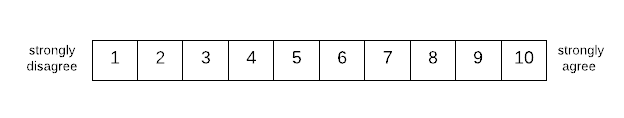
\includegraphics[width=3.5in]{Nrs-10}
		\label{Nrs}
	\end{figure}
	
	After the data collection, the rating scale will categorize the acceptability levels. Descriptive statistics will be utilized to analyze the collected data. Analysis includes calculating the minimum, maximum, mean, and standard deviation for each category. Formula \ref{mean} shows the mean that computes the average score. This use of data allows both the system functionality and its user acceptability to be comprehensively assessed. 
	
	\begin{equation} 
		\label{mean}
		\bar{x} = \frac{\sum_{i=1}^{n} x_{i}}{n}
	\end{equation}
	
	Where:
	\\$\bar{x}$ - sample mean
	\\$n$ - sample size
	\\$x_{i}$ - data points
	
	
	
	

\section{Ethical Considerations}
	Data gathered contained sensitive data so that ethical considerations should be practiced throughout the research.  Informed consent will be obtained from each participant, providing them with a clear understanding of the research purpose, procedures, and their rights to withdraw at any time. To protect the participants’ privacy, all responses will be anonymized and handled with strict confidentiality. Additionally, data usage will be restricted to research purposes only, ensuring that participants' information remains safeguarded throughout the research process and beyond. 
	
	\textbf{Informed Consent:} All respondents are informed about the purpose, procedures, and potential impacts of the study before they agree to participate. The respondents will be given a detailed explanation of the study, including the nature of their involvement, the voluntary nature of participation, and their right to withdraw at any time.
	
	\textbf{Confidentiality and Anonymity:} Personal identifiers are removed from the data to ensure that the respondents cannot be traced back to other respondents. Data are stored securely, and access will be restricted to the researchers. Any publications or presentations resulting from the study will use aggregated data with no individual responses disclosed, safeguarding the identity and privacy of all respondents.
	
	\textbf{Data Protection:} The study will adhere to relevant data protection regulations, such as local data protection laws, ensuring the secure handling and storage of all collected data. Informing the respondents about how their data will be collected, stored, and used. Their rights to privacy and data protection will be respected, and only authorized researchers will have access to the information.
	
	\textbf{Minimizing Harm:} The study will be structured to minimize any potential harm to respondents. This includes ensuring that all questions are respectful, non-discriminatory, and that the data collection process does not inconvenience the respondents. Any potential risks will be clearly communicated, and measures will be implemented to mitigate these risks and uphold the respondents well-being throughout the study.
	
	\textbf{Transparency and Honesty: } The researchers will uphold transparency and honesty throughout every stage of the study. This commitment includes accurately reporting research findings, acknowledging limitations, and strictly avoiding data manipulation or bias. Respondents will be informed of the study's progress, purposes, and outcomes, ensuring they remain fully aware of how their contributions are utilized and valued within the research.
	
	By adhering to these ethical principles, the study will safeguard respondents' rights and well-being, uphold the integrity of the research process, and enhance the credibility and reliability of its findings. This ethical approach shows trust between researchers and respondents, contributing to meaningful and responsible research outcomes.


%\nocite{*}
%--------------------------------------------------------------
% ENDMATTER of the Thesis
%--------------------------------------------------------------
%============%
% REFERENCES %
%============%

\printbibliography[heading=bibintoc,title={REFERENCES}] %<-start the bibliography
\clearpage


\begin{appendices}

	\begin{centerappendixtitle}
		% use centerappendixtitle if the supplementary materials will cover the entire page
		% input the title as usual then insert \pagebreak right after the title
		\chapter{Evaluation Results}
		\pagebreak
		
		\begin{spacing}{1.3}
		\begin{longtable}{p{12cm}cc}	
		\caption{End-Users Evaluation} \\
		\hline
		\textbf{Statement} & \textbf{Mean} & \textbf{SD} \\
		\hline
		\endfirsthead
		
		\multicolumn{3}{c}{{\tablename\ \thetable{} -- continued}} \\
		\hline
		\textbf{Statement} & \textbf{Mean} & \textbf{SD} \\
		\hline
		\endhead
                \multicolumn{2}{l}{\textit{Perceived Usefulness}} \\
                The system is modular and easy to modify with well-defined and independent components.
                & 8.60 & 1.14  \\
                The system components can be reused in other contexts with reusable libraries or modules.
                & 9.60 & 0.55  \\
                The system is easy to analyze for defects with tools to support analysis.
                & 9.20 & 0.84  \\
                The system is easy to modify and update with documented and manageable changes.
                & 9.00 & 1.00  \\
                The system is easy to test with automated testing tools available.
                & 9.80 & 0.45  \\ 
                \hline
                \multicolumn{2}{l}{\textit{Perceived Ease of Use}} \\  
                Learning to operate the system is easy for me.
                & 9.39 & 0.58  \\
                The system is easy to use.
                & 9.39 & 0.58  \\
                My interaction with the system is clear and understandable.
                & 9.43 & 0.66  \\
                I find it easy to become skillful at using the system.
                & 9.61 & 0.58  \\
                I find the system easy to operate.
                & 9.52 & 0.59  \\ 
                \hline
                \multicolumn{2}{l}{\textit{Attitude Towards Using}} \\
                I have a positive attitude towards using the system.
                & 9.52 & 0.59  \\
                I enjoy using the system.
                & 9.39 & 0.58  \\
                I am satisfied with using the system.
                & 9.52 & 0.59  \\ 
                \hline
                \multicolumn{2}{l}{\textit{Behavioral Intention to Use}} \\
                I intend to use the system regularly.
                & 9.30 & 0.70  \\
                I will continue to use the system in the future.
                & 9.30 & 0.70  \\
                I would recommend the system to others.
                & 9.61 & 0.58  \\ \hline
            
	    \end{longtable}
		\end{spacing}
        
        \pagebreak
        \begin{spacing}{1.3}
		\begin{longtable}{p{12cm}cc}
			\caption{IT Experts Evaluation} \\
			\hline
			\textbf{Statement} & \textbf{Mean} & \textbf{SD} \\
			\hline
			\endfirsthead
			
			\multicolumn{3}{c}{{\tablename\ \thetable{} -- 
			continued}} \\
			\hline
			\textbf{Statement} & \textbf{Mean} & \textbf{SD} \\
			\hline
			\endhead
			  \multicolumn{2}{l}{\textit{Functional Suitability}} \\
			  The system provides all the required functions without any missing functionalities.
			  & 9.80 & 0.45  \\
			  The functions are implemented correctly without any errors.
			  & 10.00 & 0  \\
			  The functions are appropriate for the tasks and meet user needs effectively.
			  & 9.60 & 0.55  \\ \hline
			  \multicolumn{2}{l}{\textit{Performance Efficiency}} \\
			  The system responds within acceptable time limits and maintains consistent response time under different conditions.
			  & 9.60 & 0.55  \\
			  The resource usage is within acceptable limits and the system efficiently uses available resources.
			  & 9.60 & 0.55  \\
			  The system can handle the expected load and is scalable to accommodate future growth.
			  & 9.80 & 0.45  \\ \hline
			  \multicolumn{2}{l}{\textit{Compatibility}} \\
			  The system can coexist with other systems without conflict and has no compatibility issues.
			  & 8.88 & 1.30  \\
			  The system can interact with other systems as required and data exchange between systems is seamless.
			  & 9.20 & 0.84  \\ \hline
			  \multicolumn{2}{l}{\textit{Interaction Capability}} \\
			  The purpose of the system is easily recognizable and the functions are easy to understand.
			  & 9.20 & 0.84  \\
			  The system is easy to learn for new users and there are adequate training materials available.
			  & 9.60 & 0.55  \\
			  The system is easy to operate with intuitive and user-friendly controls.
			  & 9.60 & 0.55  \\
			  The system protects users from making errors and provides clear and helpful error messages.
			  & 9.20 & 0.45  \\
			  The user interface is aesthetically pleasing with a consistent and professional design.
			  & 9.80 & 0.45  \\
			  The system is accessible to users with disabilities and includes features to support accessibility.
			  & 8.60 & 0.55  \\ \hline
			  \multicolumn{2}{l}{\textit{Reliability}} \\
			  The system is mature and stable with no frequent crashes or failures.
			  & 9.80 & 0.45  \\
			  The system is available when needed with no downtime issues.
			  & 9.00 & 0.71  \\
			  The system can tolerate faults and continue operating with mechanisms for fault detection and recovery.
			  & 9.80 & 0.45  \\
			  The system can recover from failures quickly with backup and recovery procedures in place.
			  & 9.80  & 0.45\\ \hline
			  \multicolumn{2}{l}{\textit{Security}} \\
			  The system ensures the confidentiality of data with measures to protect sensitive information.
			  & 9.60 & 0.55  \\
			  The system ensures the integrity of data with mechanisms to prevent data corruption.
			  & 9.80 & 0.45  \\
			  The system can verify the identity of users and actions are traceable to specific users.
			  & 9.20 & 0.84  \\
			  The system provides accountability for actions with maintained logs and audit trails.
			  & 9.20 & 0.84  \\
			  The system verifies the authenticity of data and users with measures to prevent unauthorized access.
			  & 8.80 & 1.30  \\ \hline
			  \multicolumn{2}{l}{\textit{Maintainability}} \\
			  The system is modular and easy to modify with well-defined and independent components.
			  & 8.60 & 1.14  \\
			  The system components can be reused in other contexts with reusable libraries or modules.
			  & 9.60 & 0.55  \\
			  The system is easy to analyze for defects with tools to support analysis.
			  & 9.20 & 0.84  \\
			  The system is easy to modify and update with documented and manageable changes.
			  & 9.00 & 1.00  \\
			  The system is easy to test with automated testing tools available.
			  & 9.80 & 0.45  \\ \hline \\
			  \multicolumn{2}{l}{\textit{Flexibility}} \\
			  The system can be adapted to different environments with configuration options available.
			  & 8.80 & 1.10  \\
			  The system can scale to meet increased demand with mechanisms to support scalability.
			  & 9.40 & 0.55  \\
			  The system is easy to install with clear and straightforward installation procedures.
			  & 10.00 & 0.00  \\
			  The system can be easily replaced with another system with procedures for system replacement in place.
			  & 9.80 & 0.45  \\ \hline
			
			\end{longtable}
		\end{spacing}
			
	\end{centerappendixtitle}
	
	\begin{centerappendixtitle}
		% use centerappendixtitle if the supplementary materials will cover the entire page
		% input the title as usual then insert \pagebreak right after the title
		\chapter{System Flow Chart}
		\pagebreak
		
		\begin{figure}[h]
			\centering
			\caption{Genetic Algorithm}
			\label{genalgoFlow}
			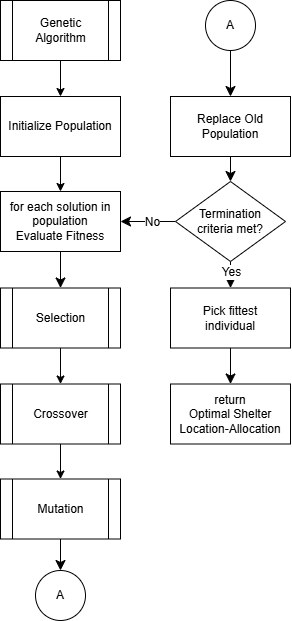
\includegraphics[width=\textwidth,height=\textheight,keepaspectratio]{appendix/Genetic Algorithm Flowchart}
		\end{figure}
		
		\begin{figure}[h]
			\centering
			\caption{Genetic Algorithm - Selection}
			\label{selectFlow}
			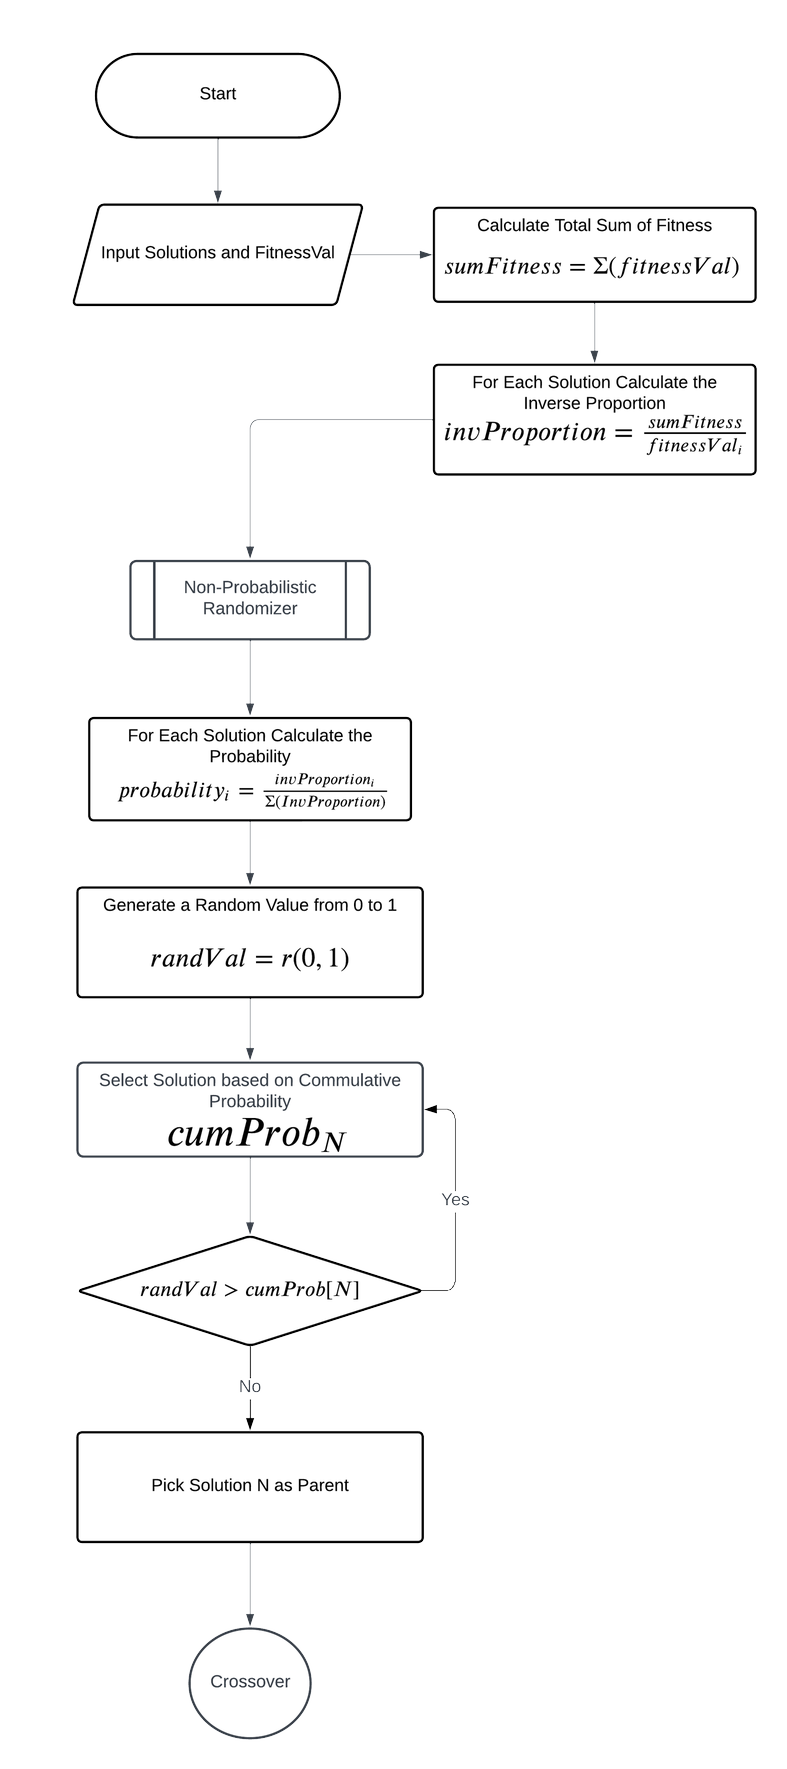
\includegraphics[width=\textwidth,height=\textheight,keepaspectratio]{appendix/select f}
		\end{figure}
		
		\begin{figure}[h]
			\centering
			\caption{Genetic Algorithm - Crossover}
			\label{crossFlow}
			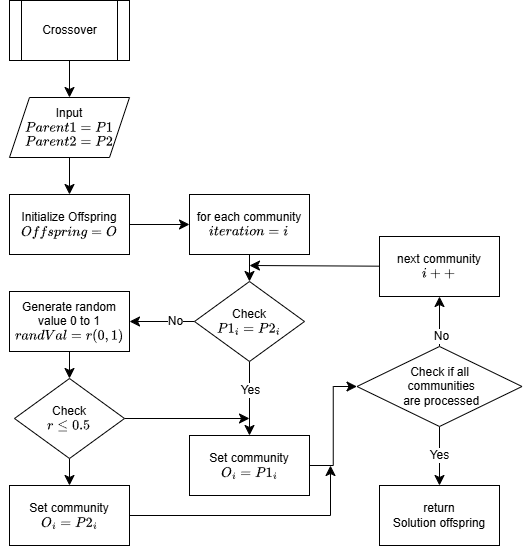
\includegraphics[width=\textwidth,height=\textheight,keepaspectratio]{appendix/crossover f}
		\end{figure}
		
		\begin{figure}[h]
			\centering
			\caption{Genetic Algorithm - Mutation}
			\label{mutateFlow}
			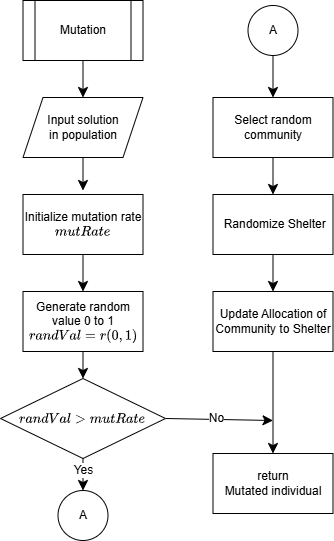
\includegraphics[width=\textwidth,height=\textheight,keepaspectratio]{appendix/mutate f}
		\end{figure}
		
		\begin{figure}[h]
			\centering
			\caption{Data Modification Feature}
			\label{dataModifFlow}
			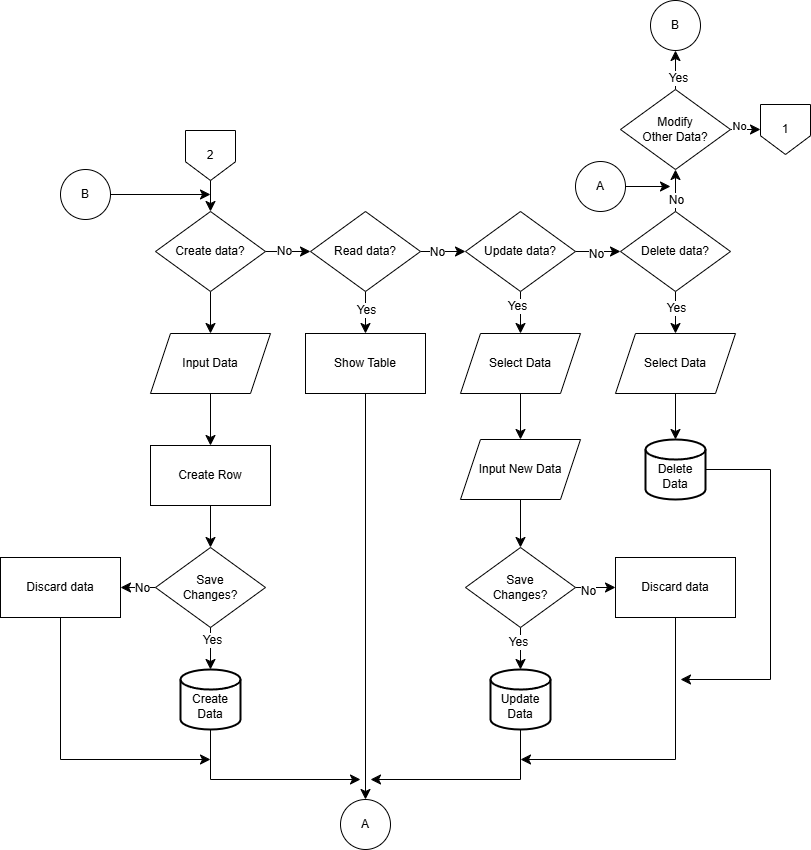
\includegraphics[width=\textwidth,height=\textheight,keepaspectratio]{appendix/data modif f}
		\end{figure}
		
		\begin{figure}[h]
			\centering
			\caption{Model Modification Feature}
			\label{modelFLow}
			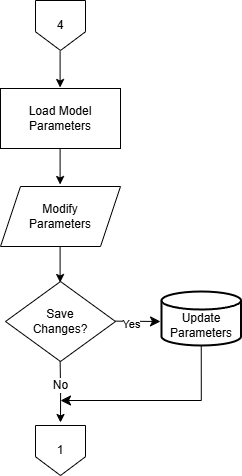
\includegraphics[width=\textwidth,height=\textheight,keepaspectratio]{appendix/modelset f}
		\end{figure}
		
		\begin{figure}[h]
			\centering
			\caption{Data Simulation Feature}
			\label{simFlow}
			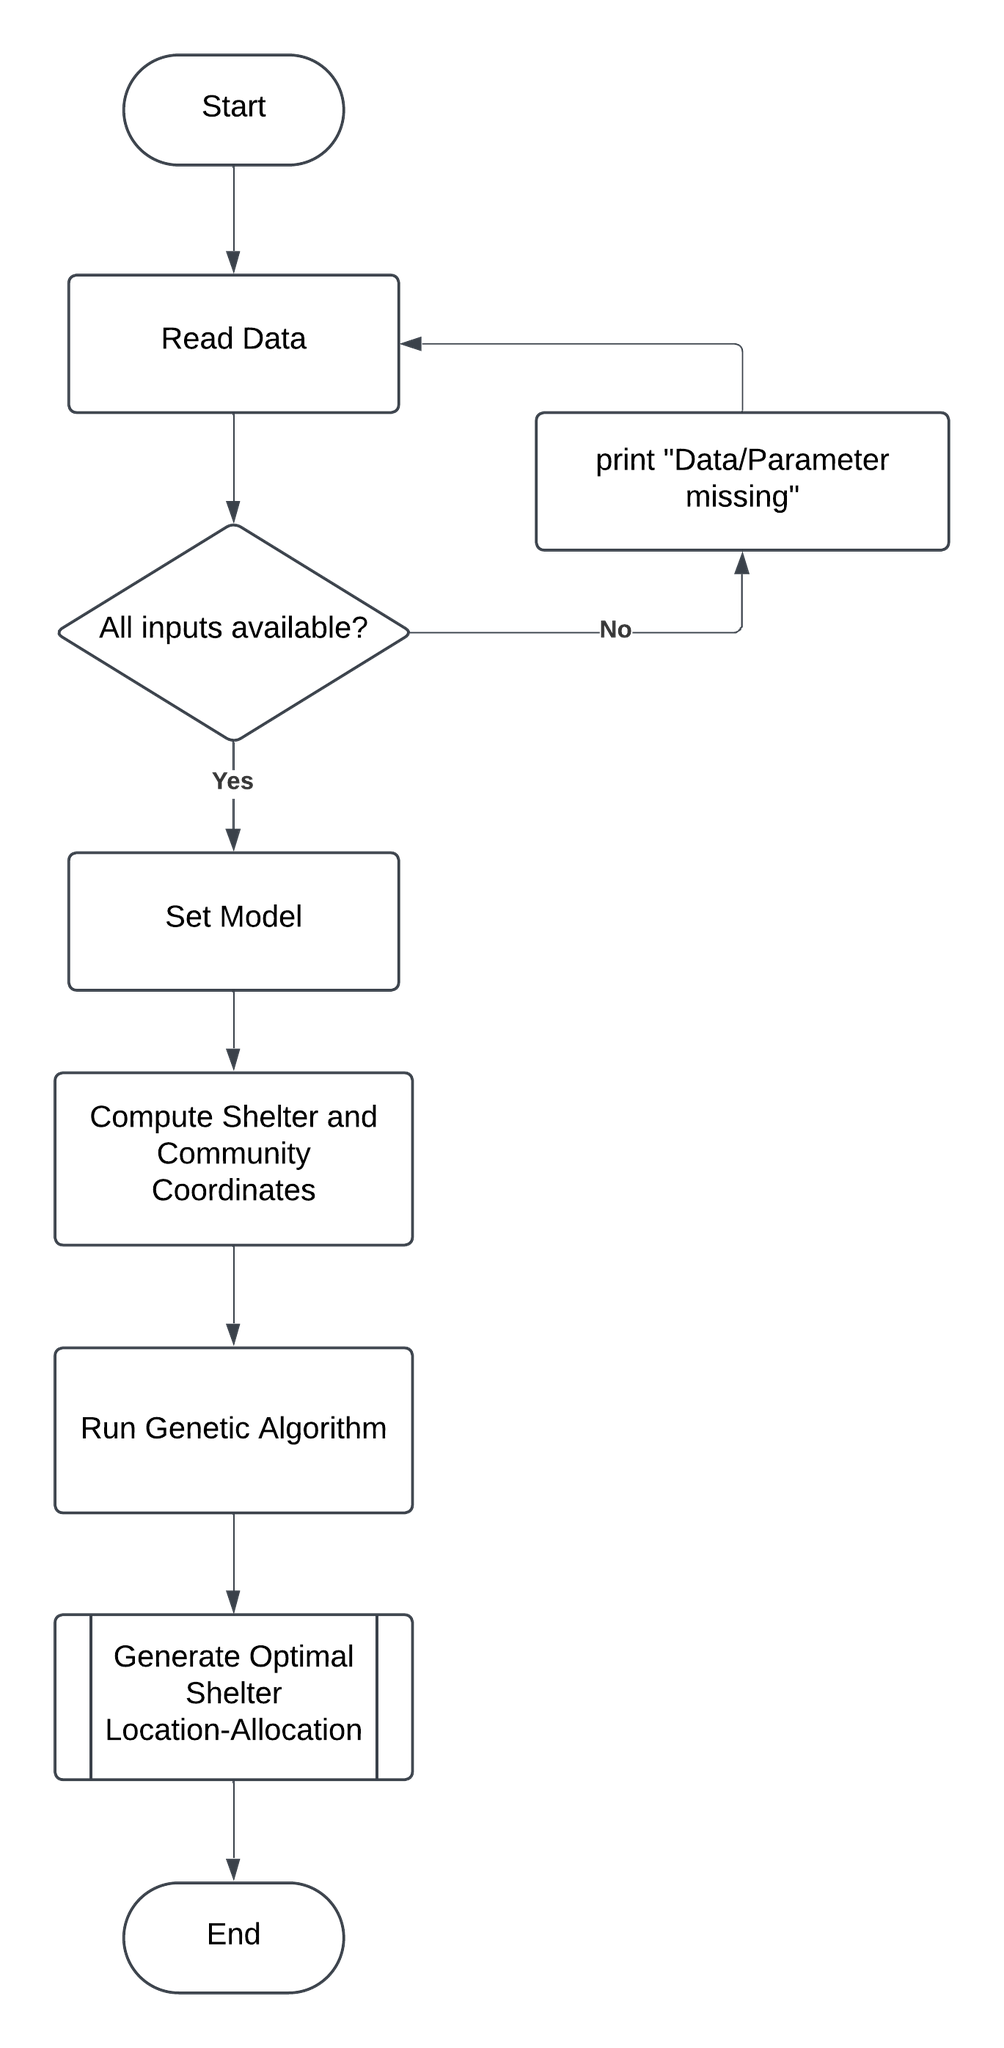
\includegraphics[width=\textwidth,height=\textheight,keepaspectratio]{appendix/datasim f}
		\end{figure}
		
		\begin{figure}[h]
			\centering
			\caption{Shelter Tagging Feature}
			\label{shelTagFlow}
			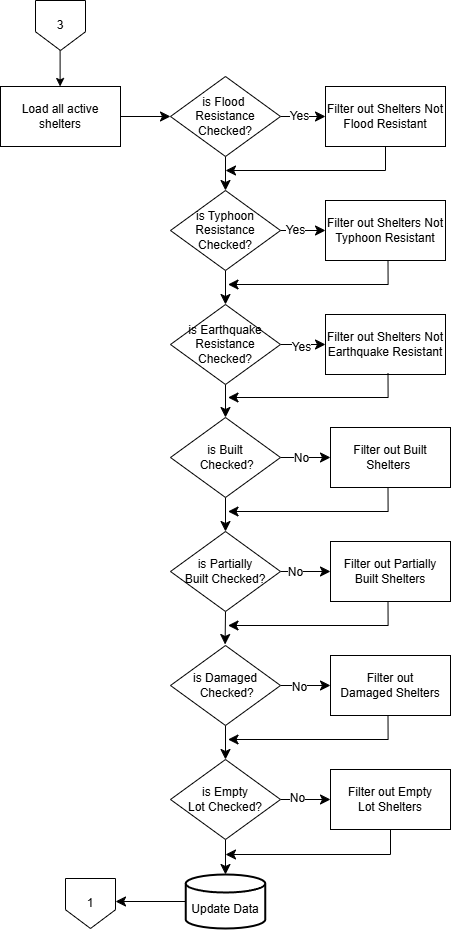
\includegraphics[width=\textwidth,height=\textheight,keepaspectratio]{appendix/sheltertag f}
		\end{figure}
		
		\begin{figure}[h]
			\centering
			\caption{Report Protection Feature}
			\label{protectFlow}
			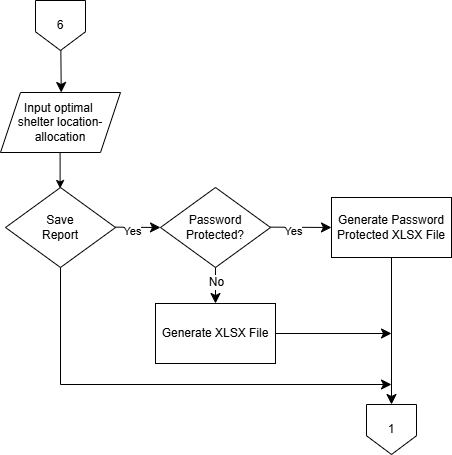
\includegraphics[width=\textwidth,height=\textheight,keepaspectratio]{appendix/protect f}
		\end{figure}
		
		
		
	\end{centerappendixtitle}
	
	\begin{centerappendixtitle}
		% use centerappendixtitle if the supplementary materials will cover the entire page
		% input the title as usual then insert \pagebreak right after the title
		\chapter{Relevant Codes}
		\pagebreak
		
		
		\begin{lstlisting}[language=Python, caption={Genetic Algorithm}, label={genalgoCode}, breaklines=true]
 generation_last_updated = 0

 for _ in range(num_solutions):
     solution = spawn()
     solutions.append(solution)

 # generations
 for generation in range(num_generations):
     # check for cancellation
     if self.cancelled:
         self.progress_dialog("Genetic algorithm cancelled.")
         return

     # sorting from best to worst solutions
     ranked_solutions = [(fitness(sol), sol) for sol in solutions]
     ranked_solutions.sort(key=lambda x: x[0]) aaaaaaaaaaaaaaaaaaaaaaaaaaaaaaaaaaaaaaaaaaaaaaaaaaa

     # initiate selection and crossover
     new_population = []
     for i in range(num_solutions):
         mother = selectParent(ranked_solutions)[1]
         father = selectParent(ranked_solutions)[1]

         offspring = generate_offspring(mother, father)
         new_population.append(offspring)

     # initiate mutation
     mutated_population = []
     for solution in new_population:
         if random.random() < mutation_rate:
             solution = mutate(solution)
         mutated_population.append((fitness(solution),solution))

     # getting the top half solutions
     best_solutions = mutated_population + ranked_solutions
     best_solutions = sorted(best_solutions, key=lambda x: x[0])[:num_solutions] 

     if (generation+1) % 100 == 0 :
         self.progress_dialog(str(best_solutions[0]))
         print(best_solutions[0])
         self.progress_dialog(f"=== Gen {generation+1} best solution ===")
         print(f"=== Gen {generation+1} best solution ===")

     prev_best_solution = fitness(solutions[0])

     # replace old population
     solutions = [sol[1] for sol in best_solutions]

     new_best_solution = fitness(solutions[0])

     #update generation_last_updated
     if(prev_best_solution != new_best_solution):
         generation_last_updated = generation+1
\end{lstlisting}
		
\begin{lstlisting}[language=Python,caption={Genetic Algorithm - Selection}, label={selectionCode}]
def selectParent(solutions):
	sum_fitness = sum(fitness for fitness, _ in solutions)
	inv_proportions = [sum_fitness/ fitness for fitness, _ in solutions]
	sum_inv_proportions = sum(inv_proportions)
	probability = [inv_proportion / sum_inv_proportions for inv_proportion in inv_proportions]
	solution_indices = np.arange(len(solutions))
	
	selected_solution = np.random.choice(solution_indices, p=probability)
	
	return solutions[selected_solution]
\end{lstlisting}

\begin{lstlisting}[language=Python,caption={Genetic Algorithm - Crossover}, label={crossoverCode}]
def generate_offspring(parent1, parent2):
    offspring = {"initial":{},"shelterlvl":{}}
    for community in Community:
        #for initial
        shelters = {parent1["initial"][community["name"]], parent2["initial"][community["name"]]} 
        
        if shelters:
            chosen_shelter = random.choice(list(shelters))
        else:
            chosen_shelter = random.choice([shelter["name"] for shelter in Shelters])

        offspring["initial"][community["name"]] = chosen_shelter

    for shelter in Shelters:

        #for shelterlvl
        levels = {parent1["shelterlvl"][shelter["name"]], parent2["shelterlvl"][shelter["name"]]} 
        
        if shelters:
            chosen_lvl = random.choice(list(levels))
        else:
            chosen_lvl = random.choice([1,2])

        offspring["shelterlvl"][shelter["name"]] = chosen_lvl

    return offspring
\end{lstlisting}

\pagebreak
\begin{lstlisting}[language=Python,caption={Genetic Algorithm - Mutation}, label={mutationCode}]
def mutate(allocation):
    new_allocations = copy.deepcopy(allocation)

    for _ in range(mutation_iteration) : 
        key_rand = random.choice(list(allocation.keys()))
        gene_to_mutate = random.choice(list(allocation[key_rand].keys()))
        current_value = allocation[key_rand][gene_to_mutate]
        
        if key_rand == "initial" or key_rand == "transferred":
            available_choices = [shelter["name"] for shelter in Shelters if shelter["name"] != current_value]
        elif key_rand == "shelterlvl":
            available_choices = [1,2]
            available_choices.remove(current_value)

        if available_choices:
            new_value = random.choice(available_choices)
            new_allocations[key_rand][gene_to_mutate] = new_value
            
    return new_allocations
\end{lstlisting}

\pagebreak
\begin{lstlisting}[language=Python,caption={Objective Value}, label={objValCode}]
def fitness(allocation):
    initial_shelters = set(allocation['initial'].values())
    Shelters_dict = {shelter["name"]: shelter for shelter in Shelters}

    total_distance = 0
    total_cost = 0

    for community in Community:
        # add distance * population
        shelter_name = allocation["initial"][community["name"]]
        distance = community["distances"][shelter_name]
        total_distance += distance * community["population"]


    for shelter_name in initial_shelters:
        # add cost based on shelter level
        shelter = Shelters_dict.get(shelter_name)
        if (allocation["shelterlvl"][shelter_name] == 1):
            total_cost += shelter["cost1"] 
        elif (allocation["shelterlvl"][shelter_name] == 2):
            total_cost += shelter["cost2"] 
        else:
            print("Shelter exceeded 2 levels. Something is wrong")
        
    # the actual model
    objective_value = weight_dist * total_distance + weight_cost * total_cost
    penalty_value = penalty_constant * getPenaltySum(allocation)

    # handle division by zero
    if objective_value + penalty_value == 0:
        return 1

    return int(objective_value + penalty_value)
\end{lstlisting}

\begin{lstlisting}[language=Python,caption={Maximum Distance Constraint}, label={maxdistCode}]
def check_max_distance(allocation):
    penalty = 0

    for community in Community:
        shelter_name = allocation["initial"][community["name"]]
        distance = community["distances"][shelter_name]
        max_distance_community = community["maxdistance"]
        # check if distance is greater than max dist
        if (distance > max_distance_community):
            print("maximum distance constraint failed")
            penalty += distance - max_distance_community
        
    return penalty
\end{lstlisting}

\pagebreak
\begin{lstlisting}[language=Python,caption={Capacity Constraint}, label={capCode}]
def check_initial_capacity(allocation):
    shelter_areas = {shelter["name"]: shelter[f"area{allocation["shelterlvl"][shelter['name']]}"] for shelter in Shelters}
    used_area = {shelter["name"]: 0 for shelter in Shelters}

    penalty = 0

    for community in Community:
        shelter_name = allocation["initial"][community["name"]]
        if shelter_name:
            # add to used_area based on population
            required_area = community["population"] * area_per_individual
            used_area[shelter_name] += required_area

            if used_area[shelter_name] > shelter_areas[shelter_name]:
                print("initial capacity constraint failed")

    for shelter in Shelters:
        shelter_name = shelter["name"]
        penalty_value = used_area[shelter_name] - shelter_areas[shelter_name]
        penalty += max(0,penalty_value)

    return penalty
\end{lstlisting}

\begin{lstlisting}[language=Python,caption={Maximum Shelter Constraint}, label={maxshelCode}]
def check_max_shelters(allocation):
    used_shelters = set() 
    penalty = 0

    for community in Community:
        shelter_name = allocation["initial"][community["name"]]
        used_shelters.add(shelter_name)  

    # If the number of unique shelters exceeds the max allowed
    if len(used_shelters) > max_shelters:
        print("max shelters constraint failed")
        penalty += len(used_shelters) - max_shelters
            
    return penalty
\end{lstlisting}

\pagebreak
\begin{lstlisting}[language=Python,caption={Maximum Level 2 Shelter Constraint}, label={maxl2shelCode}]
def check_max_lvl2_shelters(allocation):
    lvl2_shelters_ctr = sum(1 for level in allocation["shelterlvl"].values() if level == 2)
    penalty = 0

    if lvl2_shelters_ctr > max_lvl2_shelters:
        print("max lvl2 shelters constraint failed")
        penalty += lvl2_shelters_ctr - max_lvl2_shelters 

    return penalty
\end{lstlisting}
		
		
		
	\end{centerappendixtitle}
	
	\begin{centerappendixtitle}
		% use centerappendixtitle if the supplementary materials will cover the entire page
		% input the title as usual then insert \pagebreak right after the title
		\chapter{Letters}
		\pagebreak
		
		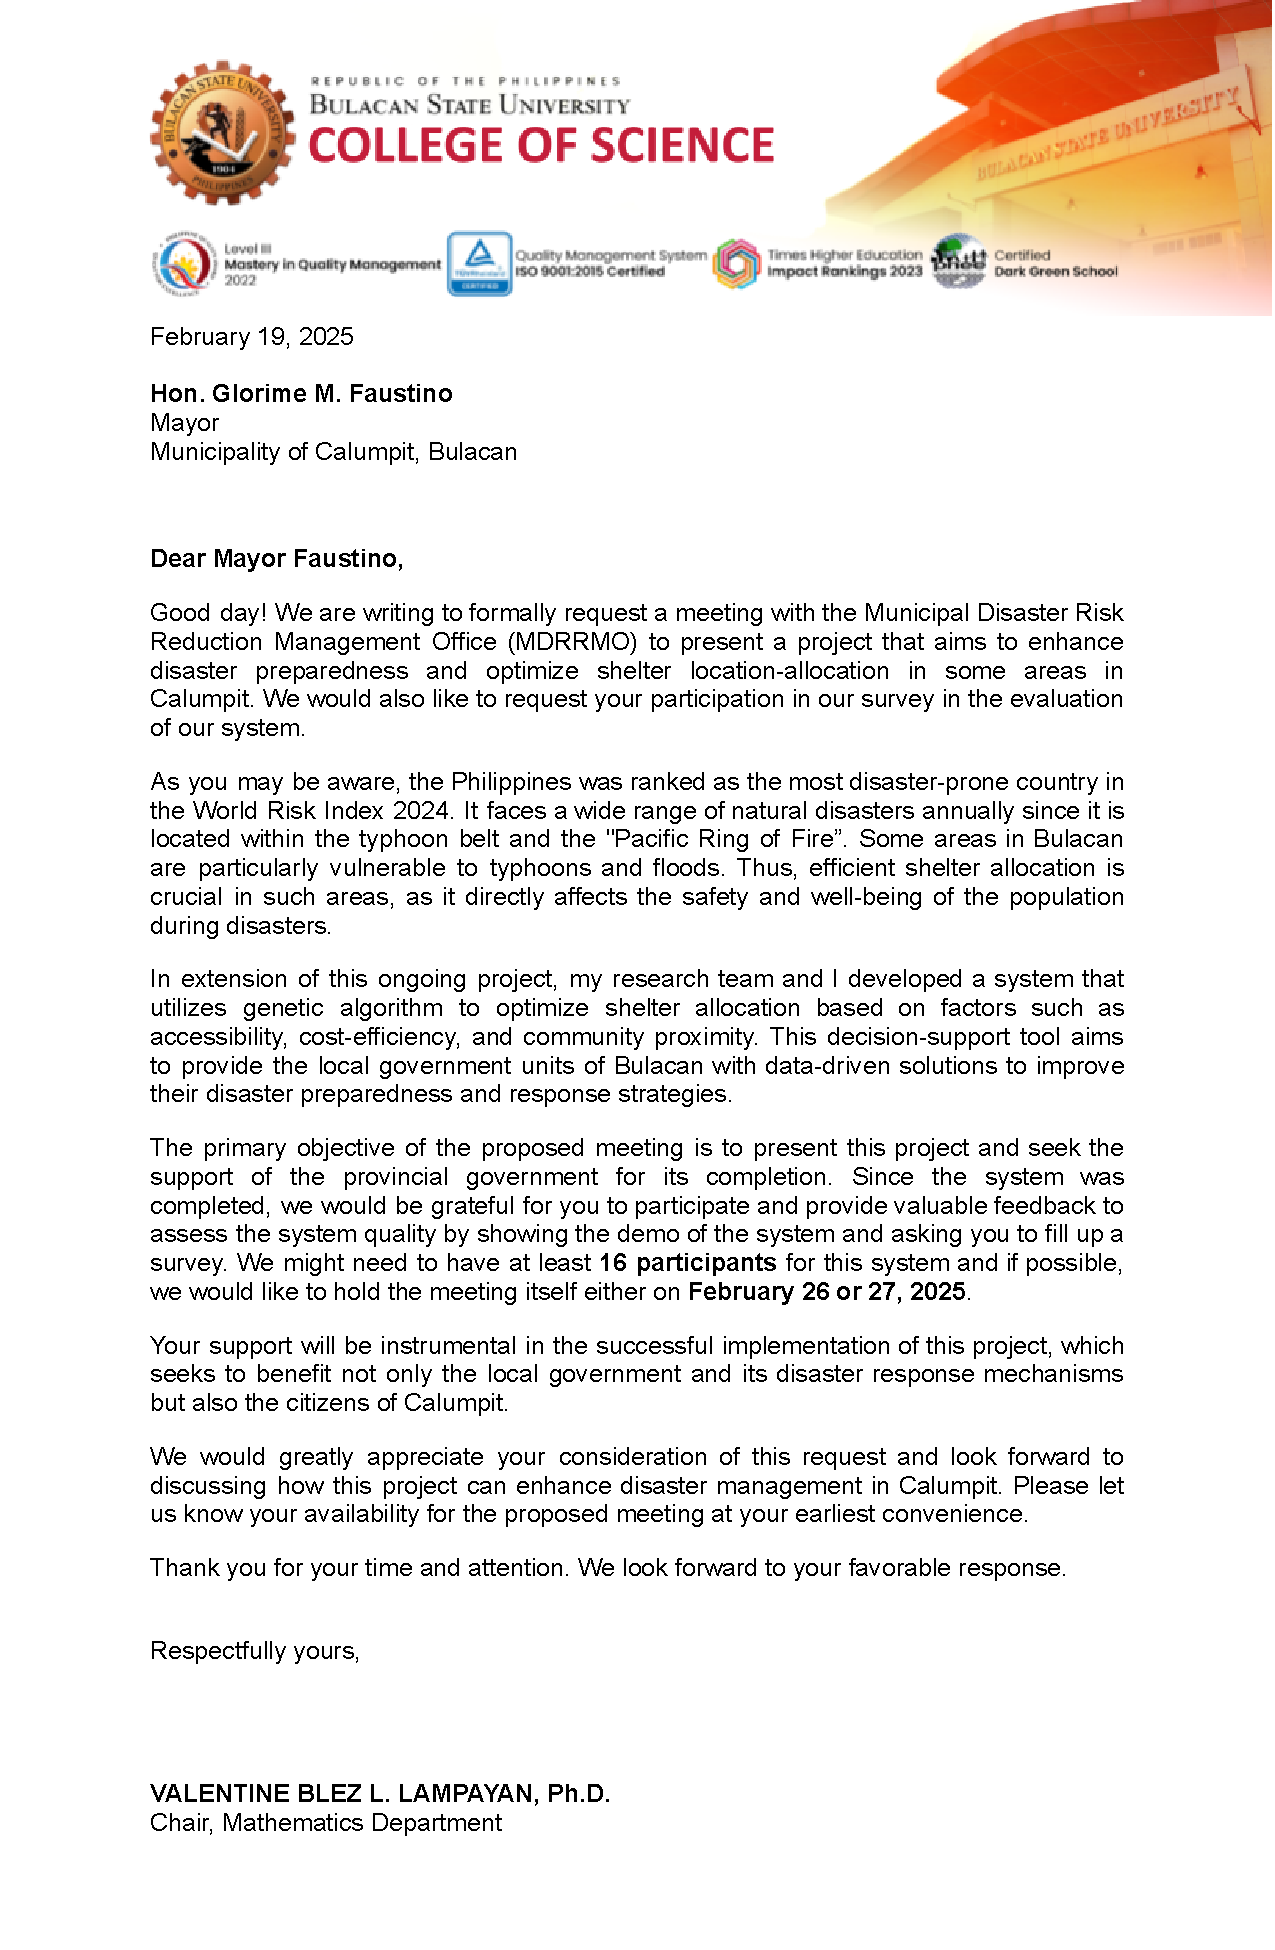
\includepdf[pages=1,pagecommand={}]{appendix/Letter-of-Intent-Research-Collab-MDRRMO-Participants}
		
\includepdf[pages=1,pagecommand={}]{appendix/Letter-of-Intent-Research-Collab-MSWDO-Participants}
		\includepdf[pages=-,pagecommand={}]{appendix/Thesis-Endorsement}
		
		
	\end{centerappendixtitle}
	
	\begin{centerappendixtitle}
		% use centerappendixtitle if the supplementary materials will cover the entire page
		% input the title as usual then insert \pagebreak right after the title
		\chapter{Instruments}
		\pagebreak
		
		
		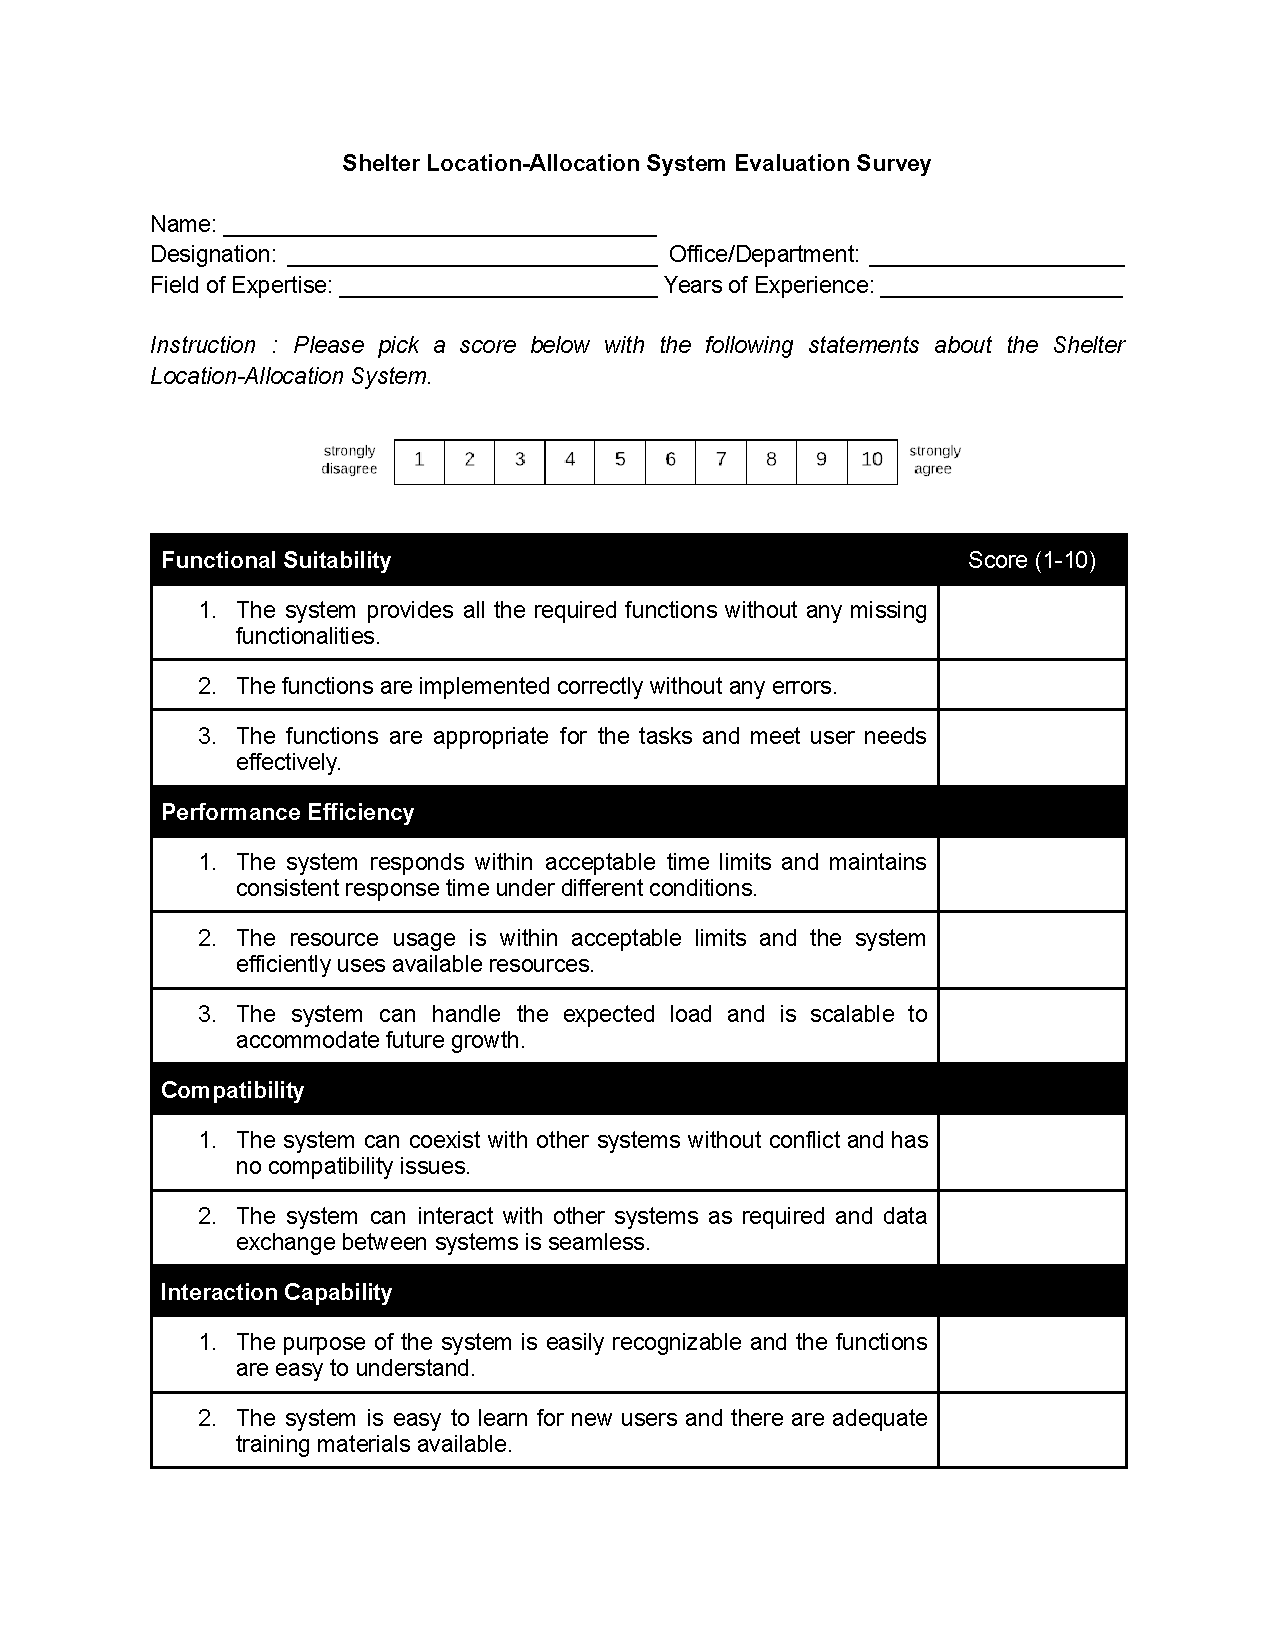
\includepdf[pages=-,pagecommand={}]{appendix/[ISOQuestionnaire]_Thesis}
		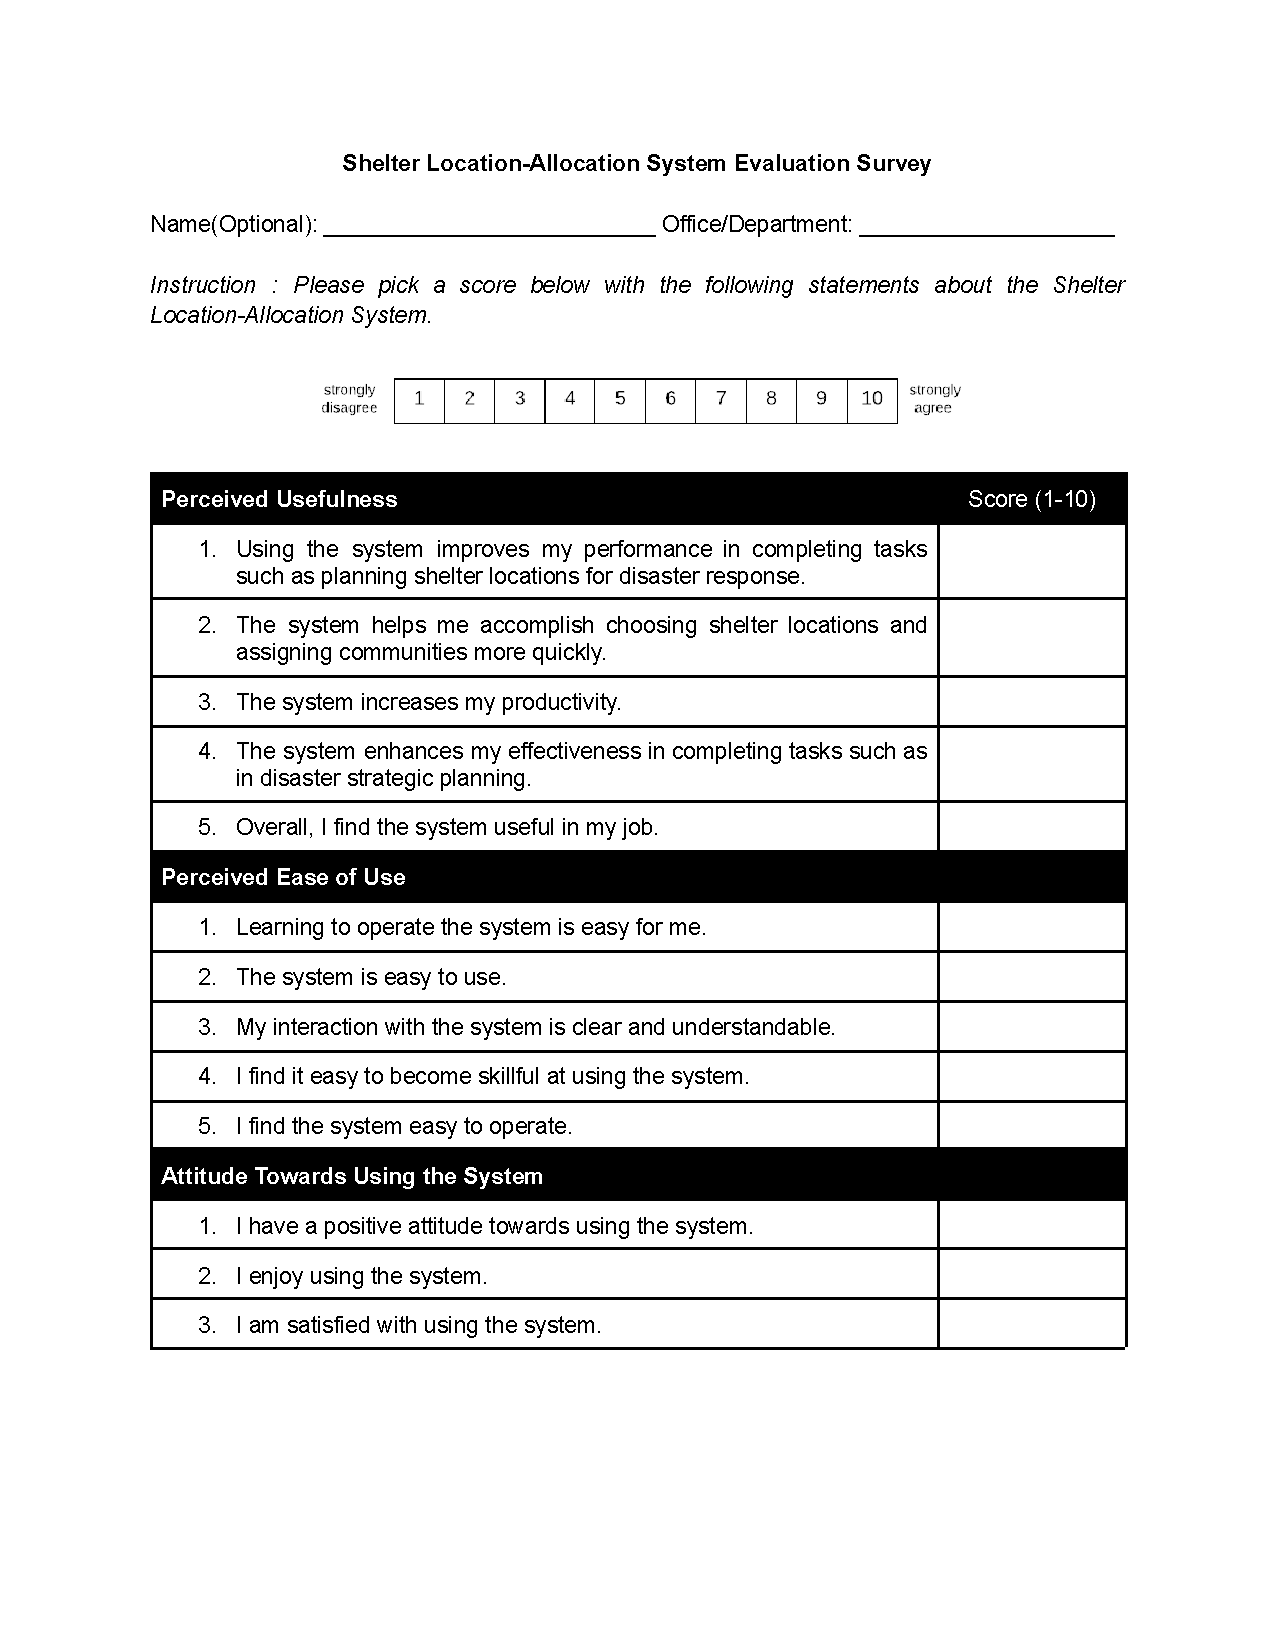
\includepdf[pages=-,pagecommand={}]{appendix/[TAMQuestionnaire]_Thesis}
	\end{centerappendixtitle}
	
	
	
\end{appendices}

\end{document}